% !TEX root = ../main.tex

\glsresetall


\topquote[10cm]{
People assume that time is a strict progression of cause to effect, \\
but, actually, from a non-linear, non-subjective point of view, \\
it's more like a big ball of... wibbily-wobbly... timey-wimey... stuff.}
{Doctor Who (David Tennant)}


{
\singlespacing
\chapter{Estimation of rare allele age}
\label{ch:rvage}
\minitoc
}


%
\section{Introduction}
%

The inference of the genealogical history of a sample is of interest to a myriad of applications in genetic research, both in population and medical genetics.
The ``age'' of an allele, which simply refers to the time since the allele was created by a mutation event, is of particular interest; for example, to observe demographic processes and events, or to better understand the effects of disease-related variants by their time of emergence in the population.

In this chapter, I propose a composite likelihood method to estimate the age of an allele, which is based on a collection of statistical models that derive from coalescent theory.
Composite likelihood methods recently have gained in popularity for various applications in genetic research.
The coalescent-based approach was pioneered by \citet{Hudson:2001vs} and has been used successfully, for example, for the fine-scale estimation of recombination rates \citep{McVean:2004ca,Myers:2005vi}.
In contrast to existing methods for allele age estimation \citep[\eg, see review by][]{Slatkin:2000us}, the method I present in this chapter does not require prior knowledge about past demographic processes or events.
Although an assumption of certain population parameters is required, such as effective population size (\Ne) or mutation rate ($\mu$), these are expected to only affect the scaling of time, such that differences between age estimates for different alleles are proportionally constant.

The age estimation framework presented in this chapter is based on allele sharing at a particular variant site observed in the sample, where the underlying IBD structure is inferred locally around the chromosomal position of the variant under consideration.
The methodology for targeted IBD detection presented in Chapters~3 and 4 is therefore essential for this approach; \ie the \texttt{tidy} algorithm which includes the \gls{fgt}, \gls{dgt}, and the probabilistic IBD model for inference using a \gls{hmm}.
I implemented the age estimation method as a computational tool written in \cpp, referred to as the \textbf{\texttt{rvage}} algorithm (for \underline{r}are \underline{v}ariant \underline{a}\underline{g}e \underline{e}stimation) which incorporates the full functionality of the previously presented \texttt{tidy} algorithm for IBD detection.\footnote{Rare variant age estimation (\texttt{rvage}): \url{https://github.com/pkalbers/rvage}}

I begin this chapter by introducing the concept of the method, which is followed by a detailed description of the statistical framework.
The method is evaluated in extensive simulation studies which consider genotype error as a source of estimation bias.
Although the method can be applied to \glspl{snp} occurring at any frequency, here, I focus on rare alleles in particular.
Finally, I present results using real data in relation to predicted variant consequences.



%
\section{Approach}
%

Consider a set of haplotypes which share a given allele by descent from a common ancestor who lived at some point in the past.
Suppose that the genealogical history of the sample is known such that the ancestral origin of the allele can be found by tracing back to the \gls{mrca} of the haplotypes that share the allele.
In a finite population, however, the \gls{mrca} is unlikely to indicate the individual in which the allele arose through mutation; therefore the actual age of the allele is expected to be older than the \gls{tmrca} of the set of haplotypes which share the focal allele.
The mutation from which the allele derived can be seen as a distinguishing event in the history of the population, immediately after which only \n{1} individual in the population carried the mutant allele.
It follows that the allele is expected to be younger than the \gls{mrca} of that \n{1} individual and any of the other contemporary individuals.
This insight is of particular interest as it suggests that the actual time of the mutation event lies somewhere in between those \n{2} points in time.

There are \n{2} main sources of information available from the data which relate to the \gls{tmrca}.
First, mutation events occur independently in each lineage and mutations accumulate along the sequence as the chromosome is passed on over generations.
Second, recombination events break down the length of the shared haplotype in each generation independently in each lineage.
The number of mutations which segregate in the \n{2} haplotypes as well as the genetic length of the pairwise shared haplotype segment can be used to infer the \gls{tmrca} of \n{2} chromosomes; \ie the time of the coalescent event at which the \n{2} lineages join.

In the following section, I derive the formulations for \n{3} estimators of the \gls{tmrca} of a pair of chromosomes, \n{2} of which are the \emph{mutation clock} and the \emph{recombination clock} model and are denoted by \ClockM and \ClockR, respectively.
The third estimator combines both the number of mutations and the genetic length of the segment; referred to as the \emph{combined clock} model, denoted by \ClockC.


%
\subsection{Coalescent time estimators}
%


The presented age estimation method is based on the computation of the posterior probability of the \gls{tmrca} of a pair of haplotypes.
It is assumed that no recombination has occurred along the sequence in the haplotype segment considered, such that the genealogical relationship between the \n{2} haplotypes does not change along the region.
This allows analysis under a coalescent process, where the posterior probability is proportional to the prior probability of the time to coalescence multiplied by the likelihood of the time given the estimator.
The derivation of the coalescent prior is described below.

Let $t$ be the number of discrete generations that separate \n{2} haplotypes in relation to the \gls{mrca}.
As shown by \citet{Tajima:1983bt}, the probability that \n{2} haplotypes are derived from \n{1} common ancestral haplotype $t$~generations in the past is
\begin{equation}
	f(t) ~=~ \frac{1}{2\Ne} \Big( 1 - \frac{1}{2\Ne} \Big)^{t-1}
	~\approx~ \frac{1}{2\Ne} \euler{-\frac{t}{2\Ne}}
\end{equation}
where \Ne is the effective population size.
The expression above relates to the probability distribution of the branch length in the underlying genealogical tree.
Further, the probability that the \n{2} haplotypes do not share an ancestral haplotype more recently than $t$~generations in the past is given by
\begin{equation}
	P(T_c \geq t) ~=~ 1 - \sum_{i=1}^{t-1} f(i) ~\approx~ \euler{-\frac{t}{2\Ne}}
\end{equation}
where $T_c$ is the time of the coalescent event.
It is convenient to use a continuous time approximation and measure time in units of ${2\Ne}$ generations, in the context of the coalescent, such that ${\tau = \sfrac{t}{2\Ne}}$
Thus, the coalescent prior can be expressed as
\begin{equation}
	\pi(t) ~\propto~ \euler{-\frac{t}{2\Ne}}
	\qquad \text{or} \qquad
	\pi(\tau) ~\propto~ \euler{-\tau}\ .
\end{equation}

The sections below describe each clock model in detail.
Recall that the \emph{breakpoints} of past recombination events are inferred for a pair of individuals, independently on the left and right-hand side of a target variant.
Under this \emph{variant-centric} approach, a given IBD segment is composed of \n{2} intervals, each delimited by the focal site and \n{1} distal breakpoint, where at least \n{1} recombination event was inferred to have occurred within each interval.
If no evidence of recombination was found on either the left or the right-hand side, a \emph{boundary~case} is recorded where the chromosomal end position is taken as a breakpoint to delimit the length of the interval.


%
\subsubsection{Mutation clock model (\ClockM)}
%

Let the physical length of the shared haplotype segment be denoted by $D$, measured in basepairs.
The sum of mutational differences observed along the segment in the pair of haplotypes is denoted by $S$.
The value of $S$ refers to the number of segregating sites in a sample of ${N=2}$~haplotypes, for which the infinite sites model is assumed without recombination; \eg see \citet{Watterson:1975ur} and \citet{Tavare:1997vra}.
Mutations are assumed to occur only once at each site in the history of the sample \citep{Kimura:1969tn}, such that $S$ reflects the total number of mutation events that have occurred along both lineages since the split from the \gls{mrca}.

Given the time of the \gls{mrca}, mutation events are Poisson distributed, as each mutation represents an independent binomial trial over a large number of sites, where each site has a small probability of mutation.
The mutation rate per site per generation is given by $\mu$.
In the coalescent, the mutation rate is scaled by population size, which is expressed by the composite mutation parameter ${\theta = 4\Ne\mu}$.
It follows that ${\theta \times D}$ is equal to the expected number of pairwise differences per coalescent time unit over the length of the segment.
Thus, the probability of observing $S$ over the distance $D$ and time $\tau$ is modelled as a Poisson process, such that ${S \sim \operatorname{Pois}(\theta D \tau)}$, for which the \gls{pdf} is defined as
\begin{equation}
	P(S \mid \theta,D,\tau) ~=~ \frac{(\theta D \tau)^S}{S!} \euler{-\theta D \tau}\ .
\end{equation}
Note that the equation above is the \emph{joint} probability of observing mutational differences at each site along the sequence.
The likelihood function for $\tau$ is proportional to the joint \gls{pdf}, but requires only those terms that involve $\tau$ and where constant terms can be dropped, such that
\begin{equation}
	\mathcal{L}(\tau \mid \theta,D,S) ~\propto~ \tau^S \euler{-\theta D \tau}\ .
\end{equation}
The posterior probability of the time to coalescence can now be written as
\begin{equation}
\begin{split}
	p(\tau \mid \theta,D,S)
	&~\propto~ \pi(\tau) ~\times~ \mathcal{L}(\tau \mid \theta,D,S) \\
	&~\propto~ \tau^S \euler{- \tau (\theta D + 1)}
\end{split}
\end{equation}
where $\pi(\tau)$ is the coalescent prior, reflecting the assumption that the expected time to a coalescent event grows exponentially back in time.


%
\subsubsection{Recombination clock model (\ClockR)}
%

In reference to the position of a focal allele that is shared by descent in \n{2} chromosomes, the length of the shared haplotype is delimited by \n{2} recombination events between the \n{2} lineages that occurred on either side of the focal position.
The recombination rate per site per generation is given by $\rho$;\footnote{Note that the literature often specifies $\rho$ as the population-scaled recombination rate and $r$ as the rate per site per generation.} again, the rate is rescaled by population size and the composite recombination parameter ${\psi = 4 \Ne \rho}$ is used.
The interval on the left and right-hand side of the focal position is distinguished by defining the distance variable $D_X$, where ${X \in \{L,R\}}$.
The genetic distance to the first recombination event is geometrically distributed along the sequence, but can be approximated by the exponential distribution if time is continuously measured and provided that \Ne is large; \eg see \citet{hein2004gene}.
The probability of observing a recombination breakpoint can therefore be modelled such that ${D_X \sim \operatorname{Exp}(\psi \tau)}$, for which the \gls{pdf} is defined as
\begin{equation}\label{eq:recprob}
	P(D_X \mid \psi,\tau) ~=~ 2 \psi \tau \, \euler{-2 \psi D_X \tau}
\end{equation}
which is equal to the joint probability of recombination between consecutive sites along the sequence.
The factor of $2$ is included to consider that recombination events occur independently in the \n{2} lineages.
Note that $D_X$ may refer to the entire length of interval if recombination rate is uniform, but it is straightforward to compute a variable recombination rate over the interval (\eg by using a genetic map) to derive the genetic length expressed in ${\psi D_X}$.

Considering \cref{eq:recprob}, the likelihood function for $\tau$ can be written as
\begin{equation}\label{eq:reclike_x}
	\mathcal{L}(\tau \mid \psi, D_X)
	~\propto~ \tau^{\mathrm{I}_X} \, \euler{-2 \psi D_X \tau}
\end{equation}
where $I_X$ is an indicator function of the detected breakpoint.
Recall that an IBD segment may extend to the end of a chromosome if no recombination occurred on \n{1} or both sides of the focal position; \ie a boundary case.
The indicator function is therefore defined as
\begin{equation*}\onehalfspacing
	\mathrm{I}_X ~=~
	\begin{cases}
    ~ 0 & \text{if boundary case on side}~X \\
    ~ 1 & \text{otherwise}\ .
  \end{cases}
\end{equation*}
Thus, to consider the intervals on both sides simultaneously by the length of the whole IBD segment, $D$, the following likelihood function is defined.
\begin{equation}\label{eq:reclike}
	\mathcal{L}(\tau \mid \psi, D)
	~\propto~ \tau^{\mathrm{I}_L + \mathrm{I}_R} \, \euler{-2 \psi D \tau}\ .
\end{equation}
As a result, the posterior probability of the time to coalescence under the recombination clock can be written as
\begin{equation}
\begin{split}
	p(\tau \mid \psi, D)
	&~\propto~
	\pi(\tau) ~\times~ \mathcal{L}(\tau \mid \psi, D) \\
	&~\propto~
	\tau^{\mathrm{I}_L + \mathrm{I}_R} \euler{- \tau (2 \psi D + 1)}\ .
\end{split}
\end{equation}
Note that the inference of recombination breakpoints does not require haplotype data; thus, the recombination clock model may provide a convenient solution if only genotype data is available.


%
\subsubsection{Combined clock model (\ClockC)}
%

Given the information available for both the mutation and the recombination clocks, the posterior probability of $\tau$ is readily calculated; see below.
\begin{equation}\label{eq:comlike}
\begin{split}
	p(\tau \mid \theta,\psi,D,S)
	& ~\propto~
	\pi(\tau) ~\times~
	\mathcal{L}(\tau \mid \theta, D, S) ~\times~
	\mathcal{L}(\tau \mid \psi, D) \\
	& ~\propto~
	\euler{-\tau} ~\times~
	\tau^S \euler{-\theta D \tau} ~\times~
	\tau^{\mathrm{I}_L + \mathrm{I}_R} \euler{-2 \psi D \tau} \\
	& ~\propto~
	\tau^{S + \mathrm{I}_L + \mathrm{I}_R} \euler{-\tau (D(\theta + 2 \psi) + 1)}
\end{split}
\end{equation}

However, it is worth to consider the following.
Both clocks, $\mathcal{T_{\!\!M}}$ and $\mathcal{T_{\!R}}$, can be consolidated by their conjugate prior distributions which, for both, is the Gamma distribution.
The \gls{pdf} of the Gamma distribution in support of $\tau$ is
\begin{equation*}
	\frac{\beta^\alpha}{\Gamma(\alpha)} \tau^{\alpha - 1} \euler{-\beta \tau}
\end{equation*}
where $\alpha$ is the shape and $\beta$ the rate parameter of the distribution.
Given the variables at hand for the combined clock, and under consideration of the coalescent prior, the parameters can be defined as ${\alpha = 1+ S + \mathrm{I}_L + \mathrm{I}_R}$ and ${\beta = D(\theta + 2 \psi) + 1}$.
Note that because $\alpha$ is an integer, the Erlang distribution can be used instead of the Gamma distribution, \eg to facilitate faster computation;
\begin{equation}\label{eq:comgamma}
\begin{split}
	P(S,L \mid \theta,\psi,\tau)
	& ~ = ~ P(S \mid \theta,D,\tau) ~\times~ P(D \mid \psi,\tau) \\
	& ~ = ~ \frac{(D(\theta + 2\psi) + 1)^{1 + S + \mathrm{I}_L + \mathrm{I}_R}}{(S + \mathrm{I}_L + \mathrm{I}_R)!} \tau^{S + \mathrm{I}_L + \mathrm{I}_R} \euler{-\tau (D(\theta + 2\psi) + 1)}
\end{split}
\end{equation}
for which the likelihood function for $\tau$ is identical to \cref{eq:comlike}.
Note that a similar derivation has been used by \citet{schroff2016}.


%
\subsection{Cumulative coalescent function}
%

Each clock model described above computes the posterior probability for \n{2} lineages to have coalesced at a particular point in time.
This is extended such that the posterior distribution of coalescent times is calculated over a continuous time prior such that the \gls{tmrca} can be derived from the \gls{cdf}.
Here, this approach is referred to as the \gls{ccf} which is defined as
\begin{equation}
	\Lambda_{ij}(t \mid \cdot) ~=~ \int_{0}^{t} p(\tau\mid\cdot)~d\tau
\end{equation}
where $t$ denotes the coalescent time prior and $i,j$ denote the \n{2} haplotypes under consideration.
The parameterisation of the clock model used is indicated by ``$\cdot$''.
In practise, the posterior probability ${p(\tau\mid\cdot)}$ is calculated from the Gamma (Erlang) distribution in each clock model, due to the conjugate relation described in the previous section.



%
\subsection{Composite likelihood estimation of mutation time}
%

Consider a sample of haplotypes and an allele shared by some of the haplotypes.
The time at which this allele was created by a mutation event is bound by the times of the \n{2} coalescent events that delimit the length of the branch on which the mutation occurred in the underlying coalescent tree; see the example provided in \cref{fig:info_age}.
The haplotypes which co-inherited the allele (\emph{sharers}) are distinguished from the other haplotypes which do not carry the allele (\emph{non-sharers}).
Thus, the sample is divided into \n{2} disjoint subsamples; let $X_c$ denote the set of chromosomes which share a given allele and $X_d$ the set of chromosomes which do not share that allele.
Importantly, all lineages in the $X_c$ subsample coalesce before any of them can coalesce with a lineage in the $X_d$ subsample.

%
%!TEX root = ../../main.tex


\begin{figure}[!htb]
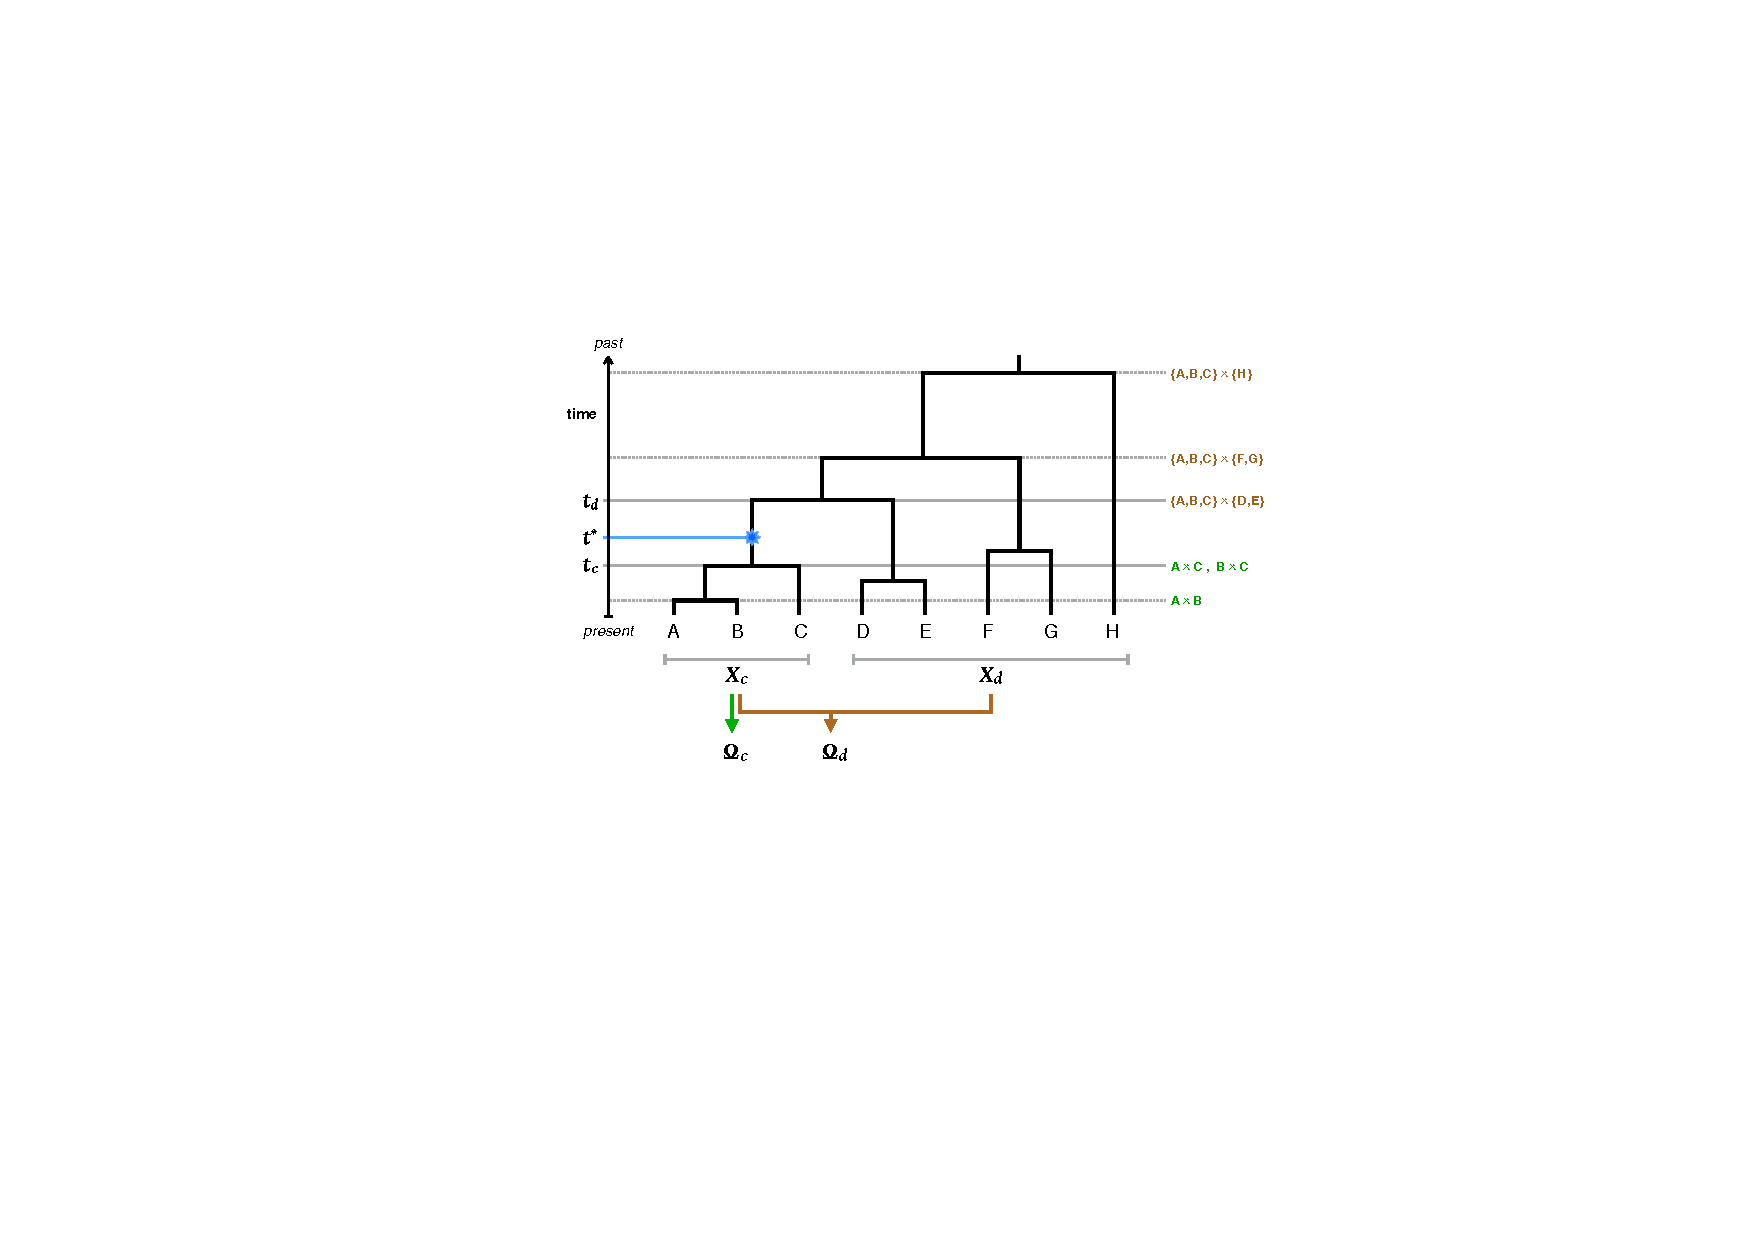
\includegraphics[width=\textwidth]{./img/ch5/info_age}
\Caption{Allele age in relation to concordant and discordant pairs}%
{The genealogy of a sample of \n{8} haplotypes is shown of which A, B, and C share a focal allele that derived from a mutation event as indicated in the tree (\emph{star}).
These chromosomes constitute the set of \emph{sharers}, denoted by $X_c$, which are differentiated from the set of \emph{non-sharers}, denoted by $X_d$.
Horizontal lines indicate the time of each coalescent event in the history of the sample within the local genealogy.
The time of the focal mutation event is denoted by ${t^\ast}$; the \n{2} coalescent events at time $t_c$ and $t_d$ define the length of the branch on which the focal mutation event occurred.
In particular, $t_c$ and $t_d$ correspond to the time until all haplotypes in $X_c$ have coalesced and the time at which the derived lineage joins the ancestral lineage of the most closely related haplotype in $X_d$, respectively.}%
{fig:info_age}
\end{figure}


% {\scriptsize \texthv{\textbf{(b)}}} \\
% \vspace{-30pt}
% \begin{center}
% \begin{tikzpicture}[-,auto,thick,
% txt/.style={font=\helvet\footnotesize,text width=4cm},
% lab/.style={font=\helvet\footnotesize,rectangle,draw=white,minimum size=0.2cm},
% sub/.style={circle,draw=white,fill=white,minimum size=0.7cm},
% con/.style={circle,draw=white,fill=oxgray!50,minimum size=0.6cm,outer sep=2pt,font=\helvet\footnotesize},
% dis/.style={circle,draw=white,fill=oxgray!50,minimum size=0.6cm,outer sep=2pt,font=\helvet\footnotesize}]
%
% \newcommand{\putConcordant}[2]{
% \node[sub] (dis#1) at (#2,1) {};
% \draw[-,draw=Brown!50,thick] (dis#1) to (conA);
% \draw[-,draw=Brown!50,thick] (dis#1) to (conB);
% \draw[-,draw=Brown!50,thick] (dis#1) to (conC);
% \node[con] (dis#1l) at (#2,1) {#1};
% }
%
% \node[txt] at (-0.5, 3.5) {$X_c$ (sharers)};
% \node[txt] at (-0.5, 1) {$X_d$ (non-sharers)};
%
%
% \node[lab,fill=ForestGreen!90] at (8, 3.775) {};
% \node[lab,fill=Brown!50] at (8, 3.275) {};
% \node[txt] at (10.25, 3.75) {Concordant pair $\in \Omega_c$};
% \node[txt] at (10.25, 3.25) {Discordant pair $\in \Omega_d$};
%
% \node[sub] (conA) at (2,3.5) {};
% \node[sub] (conB) at (4,3.5) {};
% \node[sub] (conC) at (6,3.5) {};
%
% \node[con] (conAl) at (2,3.5) {A};
% \node[con] (conBl) at (4,3.5) {B};
% \node[con] (conCl) at (6,3.5) {C};
%
% \draw [-,draw=ForestGreen!90,thick] (conA) to [out=18,in=162] (conB);
% \draw [-,draw=ForestGreen!90,thick] (conB) to [out=18,in=162] (conC);
% \draw [-,draw=ForestGreen!90,thick] (conC) to [out=144,in=36] (conA);
%
% \putConcordant{D}{1}
% \putConcordant{E}{2.5}
% \putConcordant{F}{4}
% \putConcordant{G}{5.5}
% \putConcordant{H}{7}
%
% \end{tikzpicture}
% \end{center}

%

It follows that any coalescent event between \n{2} lineages in $X_c$ must have occurred \emph{earlier} that the focal mutation event (back in time).
On the other hand, any coalescent event between \n{1} lineage in $X_c$ and \n{1} lineage in $X_d$ must have occurred \emph{later} than the focal mutation event.
In the following, pairs of haplotypes in $X_c$ are referred to as \emph{concordant} pairs and pairs from $X_c$ and $X_d$ as \emph{discordant} pairs.
The sets $\Omega_c$ and $\Omega_d$ are defined to contain all concordant and discordant pairs, respectively.

The time of a focal mutation event is found at the ``sweet~spot'' in between the earlier coalescent event at time $t_c$ and the later coalescent event at time $t_d$.
The \gls{ccf} is computed for concordant pairs in $\Omega_c$ to infer the \gls{tmrca} of the $X_c$ subsample, such that the oldest \gls{mrca} indicates the lower bound in the estimation of the focal allele age.
The upper bound is found by computing the \gls{ccf} for discordant pairs in $\Omega_d$, where the youngest \gls{mrca} is closest in time to the focal mutation event.
The information provided from these pairwise \gls{ccf} analyses are used in the calculation of the composite likelihood, which is defined below.

\begin{equation}\label{eq:compll}
	\Phi(\tau)
	~\propto~
	\prod_{i,j \in \Omega_c} \Lambda_{ij}(\tau\mid\cdot)
	\times
	\prod_{i,j \in \Omega_d} \big(1 - \Lambda_{ij}(\tau\mid\cdot) \big)
\end{equation}

The lower and upper bounds on the estimated age are provided by the incomplete gamma functions
\begin{equation}
	P_{i,j}(\tau > t) ~=~ \int_{0}^{\tau} \Phi(t \mid i,j) ~dt
\end{equation}
and
\begin{equation}
	P_{i,j}(\tau < t) ~=~ \int_{\tau}^{\infty} \Phi(t \mid i,j) ~dt \ .
\end{equation}

%
%!TEX root = ../../main.tex


\begin{figure}[!htb]
\centering
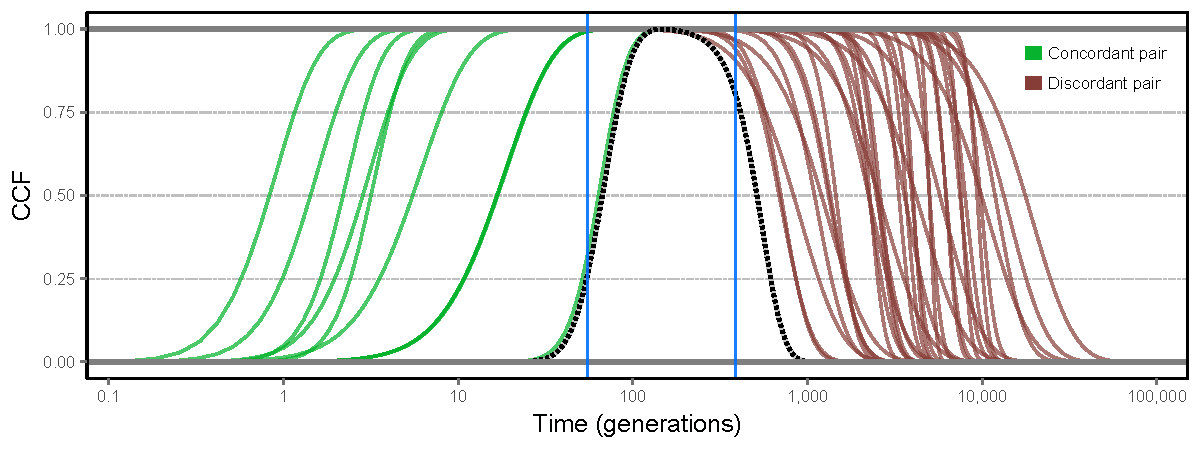
\includegraphics[width=\textwidth]{./img/ch5/age_example_new}
\Caption{Example of concordant and discordant posterior distributions and the resulting composite posterior}%
{A target variant was randomly selected from simulated data.
The \gls{ccf} was obtained for the set of possible concordant pairs and a subset of concordant pairs, which were randomly selected.
The thicker \emph{dotted} line shows the distribution of the maximised composite posterior.
The \emph{blue} lines mark the times of coalescent events below and above the focal mutation event; \ie $t_c$ (\emph{left}) and $t_d$ (\emph{right}), determined from simulation records.
Their distance corresponds to the length of the branch on which the focal mutation event occurred.}%
{fig:age_example}
\end{figure}

%

The composite likelihood estimate of the time is scaled in units of ${2 \Ne}$.
The mean, median, and mode of the posterior distribution were taken as age estimates.
In the following, the estimated age is reported using the median, which is denoted by $\hat{t}$ and expressed in units of generations.
The example shown in \cpref{fig:age_example} illustrates the output produced for a single focal variant.


%
\subsubsection{Reduction of the computational burden}
%

A major caveat to the estimation of allele age is the computationally demanding analysis of each haplotype pair in $\Omega_c$ and $\Omega_d$ per target site.
The numbers of concordant and discordant pairs are denoted by $n_c$ and $n_d$, respectively, and the overall number of pairwise analyses varies dependent on the observed frequency of the focal allele and the sample size.
For a given \fk{}~variant, the number of possible concordant pairs is
\begin{equation}\label{eq:age_nc}
	\max[n_c] ~=~ {{k}\choose{2}} ~=~ \frac{k(k-1)}{2}
\end{equation}
where $k$ is the number of allele copies observed in the sample; \ie the size of $X_c$.
The number of possible discordant pairs is given by
\begin{equation}\label{eq:age_nd}
	\max[n_d] ~=~ k(2N-k)
\end{equation}
where $N$ refers to the diploid sample size.
The total number of pairwise analyses conducted per target site is the sum of $n_c$ and $n_d$.
However, the estimation process for a single focal allele quickly becomes intractable if the allele is observed at higher frequencies or if sample size is large, which is particularly problematic if many target sites are considered.
For example, if ${N=\num{1000}}$, each \fk{2}~variant has ${n_c=2}$ and ${n_d=\num{3996}}$, whereas each \fk{20}~variant already has ${n_c=\num{190}}$ and ${n_d=\num{19600}}$.

To make the age estimation analysis computationally tractable, a sampling regime was employed which randomly pairs individual chromosomes drawn from $X_c$ and $X_d$ until a nominal threshold of unique pairs in $\Omega_c$ and $\Omega_d$ is reached.
Note that the \texttt{rvage} algorithm in its current implementation includes all possible concordant pairs in $\Omega_c$, because ${\max[n_c]}$ is assumed to be reasonably small if the focal allele frequency is low, even in larger samples of thousands of individuals.
Hence, the method specifies a sampling threshold as the upper limit of $n_d$.


%
\subsection{Inference of IBD around shared and unshared alleles}
%

The age estimation method relies on the inference of the underlying IBD structure of the sample.
In particular, IBD around a given target position is detected in each pair in $\Omega_c$ and $\Omega_d$ in order to obtain the parameter values required by the clock model used.
This is accomplished through the targeted IBD detection methodology incorporated from the \texttt{tidy} algorithm; namely the \gls{fgt}, \gls{dgt}, and the \gls{hmm}, which detect IBD in pairs of diploid individuals.
However, these methods were originally designed to detect IBD segments in individuals sharing a focal allele.
While this condition is fulfilled when considering concordant pairs, the IBD detection in discordant pairs is problematic as these are defined by not sharing the focal allele.

%
%!TEX root = ../../main.tex


\begin{figure}[!htb]
\centering
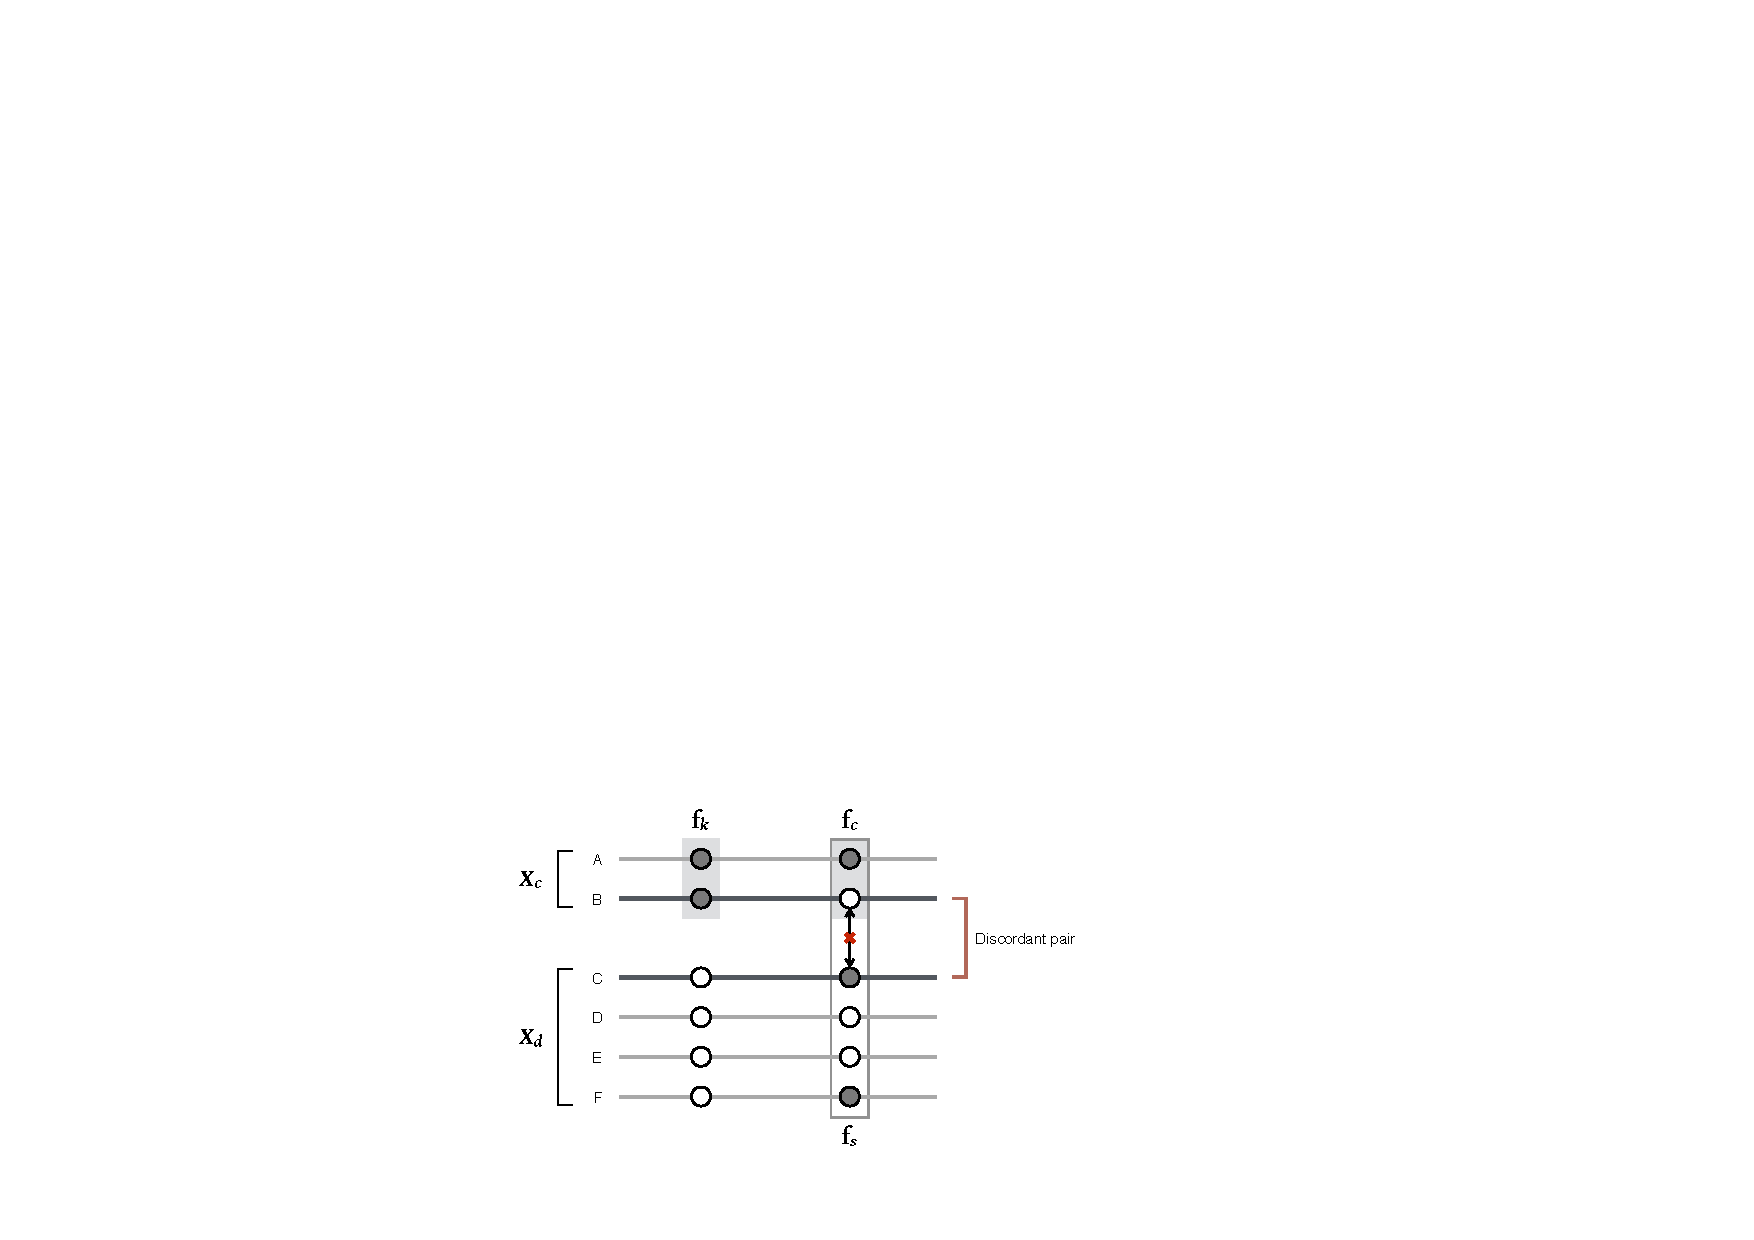
\includegraphics[width=0.7\textwidth]{./img/ch5/info_fgt_discord}
\Caption{Breakpoint detection in discordant pairs}%
{A discordant pair is formed by \n{1} haplotype from $X_c$ (which share the focal allele) and \n{1} haplotype from $X_d$ (which do not share the focal allele).
The lines indicate the chromosomal sequence where the alleles at \n{2} sites are indicated; allelic states are distinguished as the ancestral (\emph{hollow} circle) and derived state (\emph{solid}).
The conditions that lead to the detection of a recombination breakpoint is indicated between the focal site (\emph{left}) and another, distal site (\emph{right}), where \fk{} denotes the number of allele copies at the focal site within the subsample $X_c$, \fk{c} denotes the number of allele copies observed at the distal site within the subsample $X_c$, and \fk{s} denotes the number of allele copies at the distal site within the whole sample.
The \gls{fgt} is passed if all \n{4} allelic configurations are observed at \n{4} haplotypes in the sample.}%
{fig:info_fgt_discord}
\end{figure}

%

Recall that the \gls{fgt} is applied to the \n{4} haplotypes observed in \n{2} diploid individuals.
A recombination event is inferred to have occurred between \n{2} variant sites if all \n{4} possible allelic configurations are observed.
Let the focal site be denoted by $b_i$ and another, distal site by $b_j$.
In the \n{4} haplotypes, the alleles observed at ${(b_i,b_j)}$ confirm a breakpoint if, for example, ${(0,0)}$, ${(1,0)}$, ${(0,1)}$, and ${(1,1)}$ are observed, where $0$ denotes the ancestral allelic state and $1$ the derived state.
Since breakpoints are inferred on both sides of a given focal variant, the genotypes at the focal site are both heterozygous in concordant pairs.
But because the \n{2} individuals considered in a discordant pair do not share the focal allele, the required configuration cannot be observed.

To maintain the variant-centric concept, breakpoints are detected in discordant pairs as follows.
Let \fk{} denote the number of allele copies at the focal site $b_i$.
At a distal site, $b_j$, let \fk{c} denote the number of allele copies observed only within the subsample $X_c$, and \fk{s} the number of allele copies in the whole sample.
A recombination breakpoint is indicated at $b_j$ if the \n{2} haplotypes carry different alleles and if ${\fk{c} < \fk{}}$ and ${\fk{c} < \fk{s}}$; additionally ${\fk{s} > 1}$ to exclude singletons and ${(\fk{s} - \fk{c}) > (2N - \fk{})}$ to exclude sites that are monomorphic within $X_d$, where $2N$ refers to the number of haplotypes in the sample.
The condition implies the existence of the \n{4} allelic configurations at any of the haplotypes in the sample but is not bound by haplotype occurrence in \n{2} diploid individuals.
The \gls{fgt} thereby still holds but is practically inverted.
An example is illustrated in \cpref{fig:info_fgt_discord}.

Note that both the \gls{dgt} and the \gls{hmm}-based approach may operate on genotype data alone.
Importantly, if haplotype information is not available, the sets $X_c$ and $X_d$ are formed by assigning all individuals that are heterozygous to $X_c$ while all others are assigned to $X_d$, but excluding individuals that are homozygous for the focal allele.
This may reduce the information available from the sample, but the effect is expected to be negligible, in particular if the focal allele is rare.
Since haplotype data are required to determine pairwise differences, $S$, along haplotype sequences, \ClockM and \ClockC cannot be used with genotype data.

Recall that the \gls{dgt} is a special case of the \gls{fgt} which detects breakpoints at genotypic configurations that would also pass the \gls{fgt} if haplotypes were available.
Given the \n{2} heterozygous genotypes at the focal variant, a breakpoint is found at a distal site if opposite homozygous genotypes are observed; for example, ${(1,0)}$ and ${(1,2)}$, where $0$ denotes a genotype homozygous for the ancestral allele, $1$ a heterozygous genotype, and $2$ a genotype homozygous for the derived allele.
Again, in discordant pairs, such a configuration cannot be observed.
The observation of opposite homozygous genotypes nonetheless implies that the \n{2} individuals do not share a haplotype at this site and is therefore also applied for breakpoint detection in discordant pairs.

%
%!TEX root = ../../main.tex


\begin{figure}[!htb]
\centering
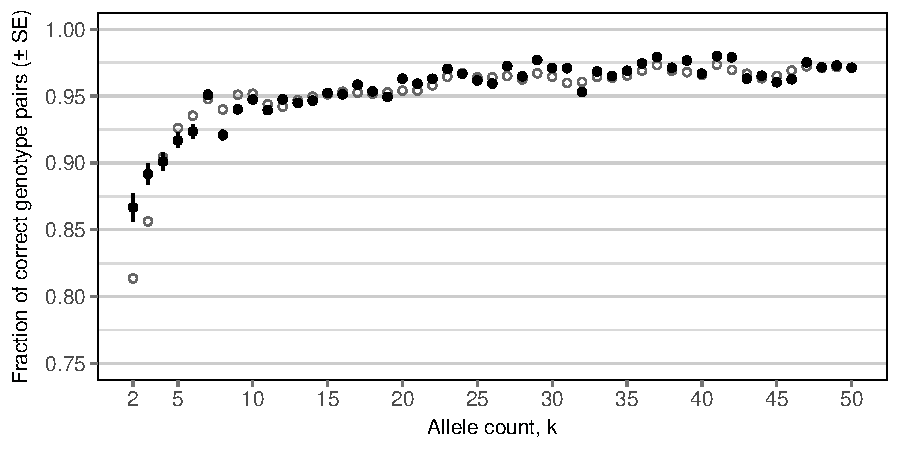
\includegraphics[width=0.8\textwidth]{./img/ch5/info_hmm_discord}
\Caption{Initial state probability of discordant pairs in the Hidden Markov Model (HMM)}%
{The proportion of discordant pairs that were correctly identified by their genotypes was empirically determined from data before and after the inclusion of realistic genotype error rates.
The mean per \fk{} was used as the initial state probability of the \gls{hmm}-based approach for IBD detection around target sites.
For comparison, the initial state probability of concordant pairs is shown (\emph{hollow} circles).}%
{fig:info_hmm_discord}
\end{figure}

%

The \gls{hmm}-based approach includes a probabilistic model for observing each possible genotype pair in pairs of diploid individuals in \emph{ibd} and \emph{non}, which are the hidden states defined in the underlying IBD model; see Chapter~4.
Both the emission and initial probabilities were determined empirically, from data before and after the inclusion of realistic genotype error rates.
The initial state probability corresponds to the probability of correctly observing a concordant pair by allele sharing, \ie the true positive rate of observing heterozygous genotypes at a given target site where both individuals share the focal allele, which was determined per focal allele frequency (\fk{}).
To extend the model to consider discordant pairs, here, initial state probabilities were estimated as the true positive rate of observing the focal allele as a heterozygous genotype in the $X_c$ individual and not observing the focal allele in a homozygous genotype, $g_0$, in the $X_d$ individual; again, based on the comparison between genotype data before and after error (using the same dataset as available in Chapter~4).
For each \fk{}~category, I randomly selected \n{1000} target sites in the dataset before error and randomly selected \n{1000} discordant pairs per target site, which I then compared to the genotypes observed in the dataset after error to determine the true positive rate.
The mean per \fk{} was taken as the empirical initial state probability.
The resulting probability distribution is shown in \cpref{fig:info_hmm_discord}; the initial state probabilities used for discordant pairs are indicated for comparison.
Notably, the discordant probability of initialisation is similar to the concordant one.
A possible explanation is that this is particularly driven by the heterozygous status being false.



%
\subsubsection{Anticipated limitations}
%

Since the estimation of allele age is dependent on parameters inferred from the underlying IBD structure of the sample, the accuracy of IBD detection is expected to affect the accuracy of the estimated age.
%
%!TEX root = ../../main.tex


\begin{figure}[p]
\centering
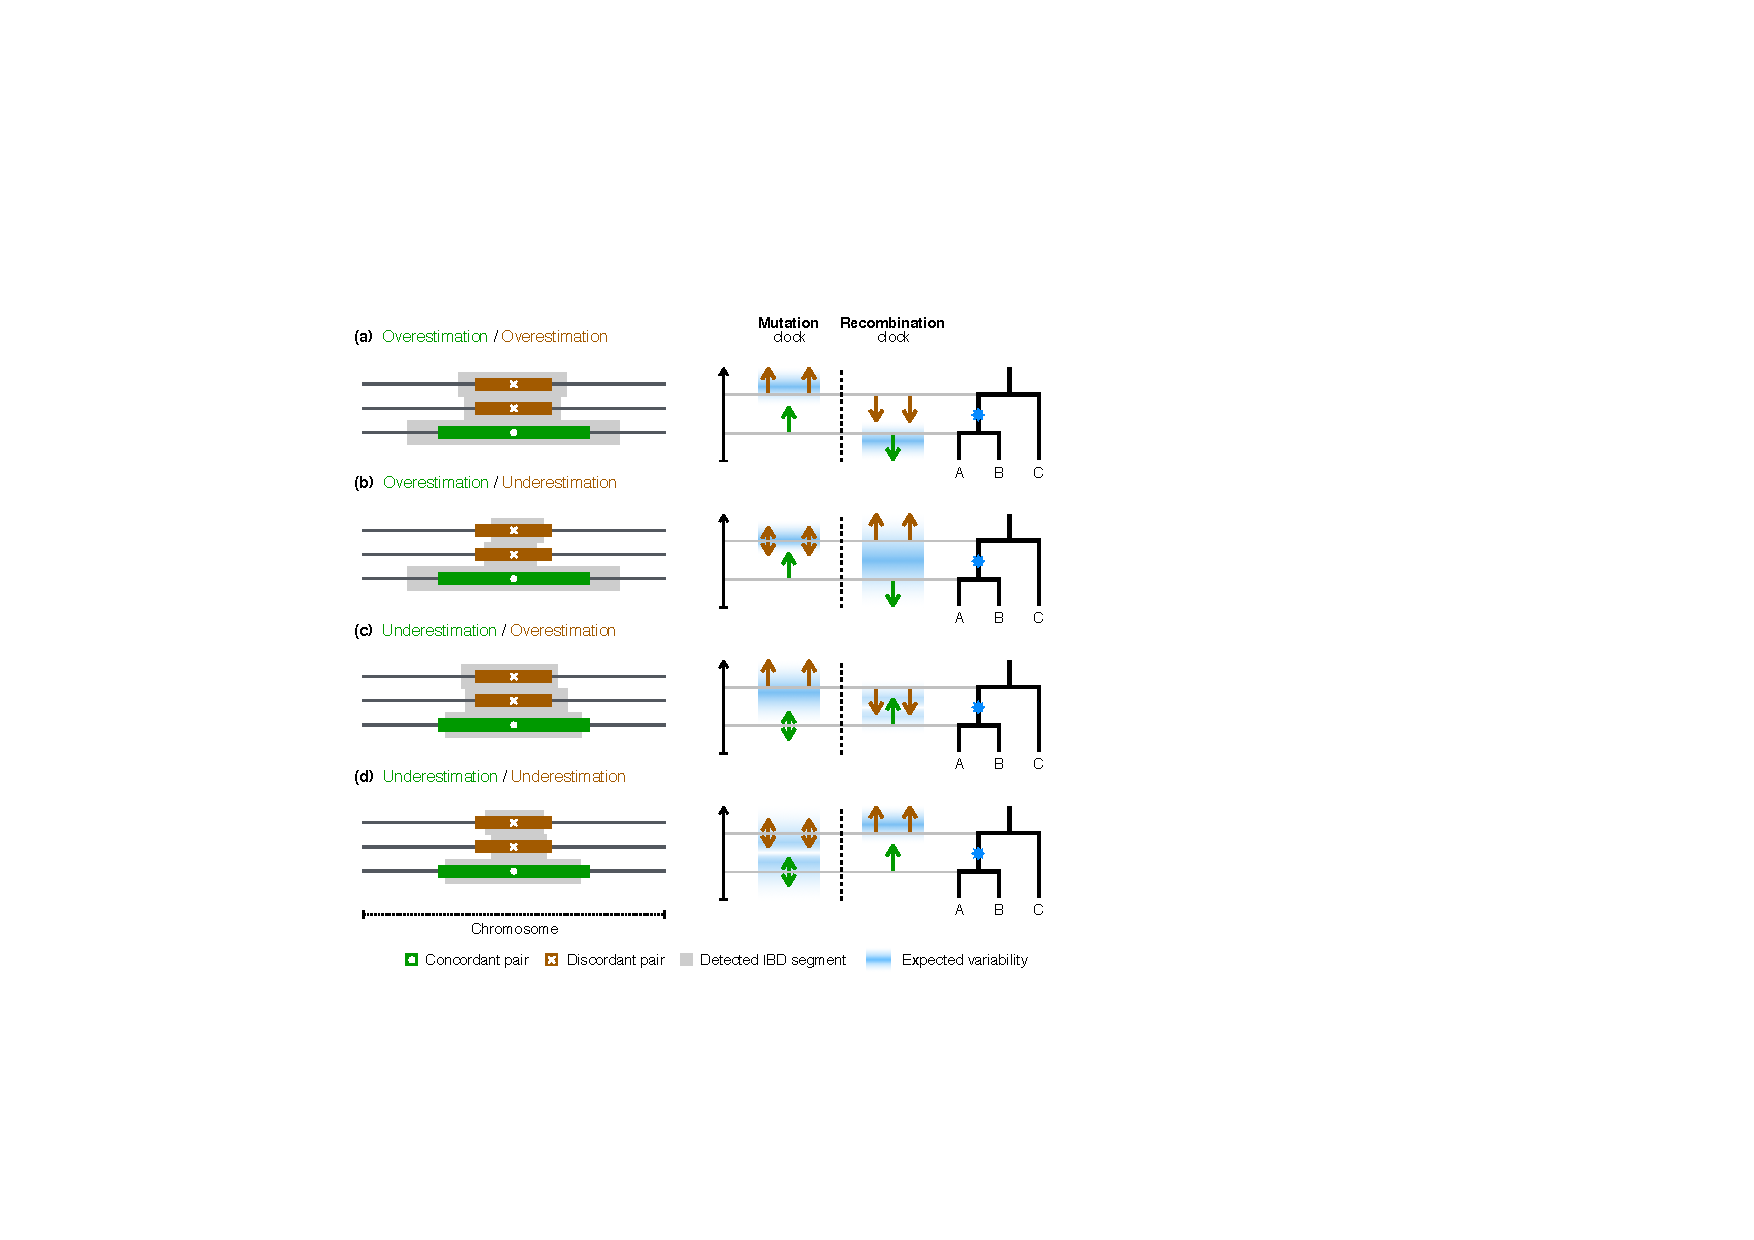
\includegraphics[width=\textwidth]{./img/ch5/info_age_bias}
\Caption{Expected estimation bias due to deficient IBD inference}%
{A minimal example is illustrated for a sample of \n{3} chromosomes where ${A,B \in X_c}$ and ${C \in X_d}$.
The focal mutation event is indicated in the genealogy of the sample (\emph{star}).
Each pair shares some haplotype region identical by decent, where the actual extent of the underlying IBD segment is shown for the concordant pair ${\{A,B\}}$ and the discordant pairs ${\{A,C\}}$ and ${\{B,C\}}$; indicated by \emph{green} and \emph{brown} bars, respectively.
The allele shared in concordant pairs is indicated (\emph{circle}), as well as the absence of allele sharing in discordant pairs (\emph{cross}).
Inferred IBD segments are shown as \emph{grey} bars at each true IBD segment, which may overestimate or underestimate the actual shared haplotype length.
Panels~\textbf{(a)} to \textbf{(d)} illustrate the possible cases of over and underestimation when observed in concordant and discordant pairs.
The arrows shown in relation to the times of coalescent events in the genealogy indicate the  direction to which the estimation under a given clock model is expected to tend, given the respective pattern of over and underestimation in concordant and discordant pairs.
The expected variability of the estimated age posterior distribution is indicated (\emph{blue}).
Note that only the mutation clock, \ClockM, and the recombination clock, \ClockR, are shown because \ClockC is a combination of both models.}%
{fig:info_age_bias}
\end{figure}
%
%
Possible consequences of inaccurately inferred lengths of IBD segments are summarised in \cpref{fig:info_age_bias}, which illustrates a minimal example for the different cases possible when concordant or discordant IBD length is over or underestimated.
For instance, in cases where IBD is overestimated in both concordant and discordant pairs (\cref{fig:info_age_bias}{a}), both the the genetic length and the number of pairwise differences, $S$, may be inflated, which affects the computation of the \gls{ccf} under the mutation and recombination clock differently.
Notably, because the pairwise probability distributions computed by the \gls{ccf} in the set of pairs are multiplied to calculate the composite likelihood in \cref{eq:compll}, it is possible that some analyses my return invalid results, as probabilities may cancel out or become too small to be distinguishable from zero given machine limits.
In the following, the term \emph{conflict} is used to refer to sites at which the analysis returned an invalid age estimate.


%
\section{Evaluation}
%

The method was assessed using data generated in coalescent simulations.
First, the validity of the method under each clock model was demonstrated based on the true IBD structure of the sample as known from simulation records.
Second, the analysis was repeated for each IBD detection method.
Third, each approach was then assessed with regard to genotype error, which also considered the effects of phasing error.


%
\subsection{Data generation}
%

The performance of the age estimation method was evaluated using several simulated datasets.
First, sample data were simulated under a simple demographic model of constant population size (${\Ne = \num{10000}}$) with mutation rate ${\mu = \num{1e-08}}$ per site per generation and constant recombination rate ${\rho = \num{1e-08}}$ per site per generation, using \texttt{msprime} \citep{Kelleher:2016fn}.
Note that by setting the mutation and recombination rates to constant and equal values, the physical and genetic lengths are identical when measured in \gls{Mb} and \gls{cM}, respectively.
The size of the simulated dataset was \n{2000} haplotypes, which were randomly paired to form a sample of ${N = \num{1000}}$ diploid individuals.
The length of the simulated region was \SI{100}{\mega\basepair} (\SI{100}{\centi\morgan}), resulting in \n{326335}~variant sites.
This dataset is denoted by $\mathcal{D}_A$.

Second, the dataset simulated in Chapter~3 was included here to evaluate the age estimation method in presence of genotype error.
Briefly, the simulation was performed under a demographic model that recapitulates the human expansion out of Africa; following \citet{Gutenkunst:2009gs}.
A sample of \n{5000} haplotypes was simulated with ${\Ne = \num{7300}}$, a mutation rate of ${\mu = \num[round-precision=2]{2.35e-8}}$ per site per generation, and variable recombination rates taken from human chromosome~20; Build~37 of the \gls{hapmap} Phase~\rom{2} \citep{Frazer:2007kha, InternationalHapMapConsortium:2010en}, yielding \dec{0.672847}~million segregating sites over a chromosomal length of \SI{62.949301}{\mega\basepair} (\SI{108.26675653}{\centi\morgan}).
The simulated haplotypes were randomly paired to form a sample of ${N = \num{2500}}$ diploid individuals.
Haplotype data were converted into genotypes and subsequently phased using \texttt{SHAPEIT\,2} \citep{Delaneau:2008dk,Delaneau:2013hi}.
Here, this permitted the assessment of the impact of phasing error on the age estimation process.

Third, the dataset described above was retrofitted in Chapter~4 to include realistic proportions of empirically estimated error, which was equally distributed in the derived genotype and haplotype datasets.
Here, data \emph{before} and \emph{after} the inclusion of error are distinguished by referring to dataset $\mathcal{D}_B$ and dataset $\mathcal{D}_B^{\ast}$, respectively.
Note that in the following the term \emph{genotype error} is used, even in analyses that operate on haplotype data, as error proportions were estimated from misclassified genotypes (see Chapter~4).

In each dataset, simulation records were queried to determine the underlying IBD structure of each pair of individuals analysed in this work.
Note that the simulated genealogy underlying $\mathcal{D}_B$ was identical to $\mathcal{D}_B^{\ast}$, such that direct comparisons were possible between results obtained before and after error.
True IBD intervals were found in simulated genealogies by scanning the sequence until the \gls{mrca} of a given pair of haplotypes changed, on both sides of a given target position.
Interval breakpoints were identified on basis of the observed variant sites in the sample, such that the resulting true IBD segment defined the smallest interval detectable from available data.
Note that this allowed overestimation of the actual genetic length of the IBD segment, but thereby provided a realistic benchmark for comparisons with IBD detection methods; namely the \gls{fgt}, \gls{dgt}, and the \gls{hmm}-based approach as implemented in the \texttt{rvage} algorithm.


%
\subsection{Accuracy analysis}
%

Coalescent simulators may not define the exact time point at which a mutation event occurred, because mutations are independent of the genealogical process (if simulated under neutrality) and can therefore be placed randomly along the branches of the simulated tree; \ie mutation times are not specified in \texttt{msprime}, but the times of coalescent events are recorded.
In simulations, the probability of placing a mutation on a particular branch is directly proportional to its length, which itself is delimited by the time of the coalescent event below (joining the lineages that derive from that branch) and the time of the coalescent event above (joining that branch with the tree back in time).
Here, the times of coalescence below and above a particular mutation event are denoted by $t_c$ and $t_d$, respectively, against which the accuracy of the estimated allele age is measured.

Although the true time of a mutation event was not known from the simulations performed, an indicative value for the age of an allele was derived from the logarithmic ``midpoint'' (or \emph{log-average}) between coalescent events, which is denoted by $t_m$ and calculated as the geometric mean of $t_c$ and $t_d$; see below.
\begin{equation}
	t_m ~=~
	\exp \bigg[ \log \big[ t_c \big] + \frac{1}{2} \bigg( \log \big[ t_d \big] - \log \big[t_c \big] \bigg) \bigg] ~=~
	\sqrt{~t_c ~ t_d~}
\end{equation}

Accuracy was measured using Spearman's rank correlation coefficient, $r_S$, which is a robust measure for the strength of the monotonic relationship between \n{2} variables; \ie the inferred allele age ($\hat{t}$) and true time proxies ($t_c$, $t_m$, or $t_d$).
Note that the squared Pearson correlation coefficient, $r^2$, was used in previous chapters but is less suitable here, as both the inferred and true age are expected to vary on log-scale, and the Pearson coefficient measures the linear relationship between variables..
In addition, the \gls{rmsle} was calculated as a descriptive score for the magnitude of error (here defined on $\log_{10}$).

To better illustrate the distribution of age estimates obtained in an analysis, the \emph{relative age} was computed, $\hat{t}_\textit{rel}$, for each allele by normalising the time scale conditional on the time interval between the coalescent events at $t_c$ and $t_d$, such that age estimates were ``mapped'' on the same scale relative to the branch length spanned between $t_c$ and $t_d$; this was calculated as below.
\begin{equation}\label{eq:age_relative}
	\hat{t}_\textit{rel} ~=~
	\frac{ \log \big[ \frac{\hat{t}}{t_c} \big] }{ \log \big[ \frac{t_d}{t_c} \big] }
\end{equation}
As a result, the times of coalescent events at $t_c$ and $t_d$ are mapped to 0 and 1, respectively.
An age estimate is defined as being ``correct'' if ${t_c \leq \hat{t} \leq t_d}$, which is equal to the condition ${0 \leq \hat{t}_\textit{rel} \leq 1}$, such that ${\hat{t}_\textit{rel} < 0}$ indicates underestimation and ${\hat{t}_\textit{rel} > 1}$ overestimation in relation to the true interval in which the mutation event could have occurred.


%
\section{Results}
%

In each dataset, \n{10000}~rare variants were randomly selected as target sites for estimation of allele age.
These were selected at shared allele frequency~${\leq \SI{1}{\percent}}$, \ie \fk{[2,20]}~variants, in $\mathcal{D}_A$.
Identical sets of target sites were randomly selected in $\mathcal{D}_B$ and $\mathcal{D}_B^{\ast}$, at shared allele frequency ${\leq 0.5\%}$ (\fk{[2,25]}~variants).
Note that these were sampled from the subset of variants unaffected by genotype error, to ensure that alleles correctly identified haplotype sharing.


%
\subsection{Validation of the method under different thresholds}
%

Because an exhaustive analysis of all possible discordant pairs becomes computationally intractable, it is convenient to reduce the number of pairwise analyses that are conducted per target allele.
For example, although the sample size of dataset $\mathcal{D}_A$ was modest (${N = \num{1000}}$), the total number of possible pairwise analyses for the set of \n{10000} selected rare variants would have been \dec{145.724783}~million.
For realistic applications of the method, it is therefore essential to limit the number of discordant pairs, $n_d$, such that ${\Omega_d}$ consists of a substantially smaller set of randomly formed pairs.
In this section, I analyse the impact on the accuracy of estimated allele age under different nominal thresholds of $n_d$ (listed below).
Importantly, to focus on the impact resulting from different $n_d$ thresholds, the analysis was conducted using true IBD segments as determined from simulation records.
Thus, this section provides a general validation analysis of the age estimation method.

\begin{center}
\begin{tabular}{r@{\hskip 2em}r}
{$n_d$} &
{Pairwise analyses} \\
	\midrule
	\num{10}   & \dec{0.461842} million \\
	\num{50}   & \dec{0.861842} million \\
	\num{100}  & \dec{1.361842} million \\
	\num{500}  & \dec{5.361842} million \\
	\num{1000} & \dec{10.366135} million \\
\end{tabular}
\end{center}

Each clock model was considered separately and the same set of \n{10000} target sites was analysed under each threshold.
This resulted in a total of \dec{276.1326}~million pairwise analyses in this section alone.
None of the analyses returned conflicting results; recall that \emph{conflicts} were defined as invalid estimates resulting from erroneous patterns of coalescent times as computed through the \gls{ccf} for the set of pairs considered.
Note that discordant pairs were formed randomly and therefore differed in each analysis.
The results are illustrated in \cpref{fig:discords_scat}, which shows the density of true and estimated age under each clock model; results are shown for ${n_d = \num{10}}$, ${n_d = \num{100}}$, and ${n_d = \num{1000}}$, to better distinguish differences visually.
Note that true age is set at $t_m$, but $t_c$ and $t_d$ are indicated in \cref{fig:discords_scat}.

%
% !TEX root = ../../main.tex


\begin{figure}[p]
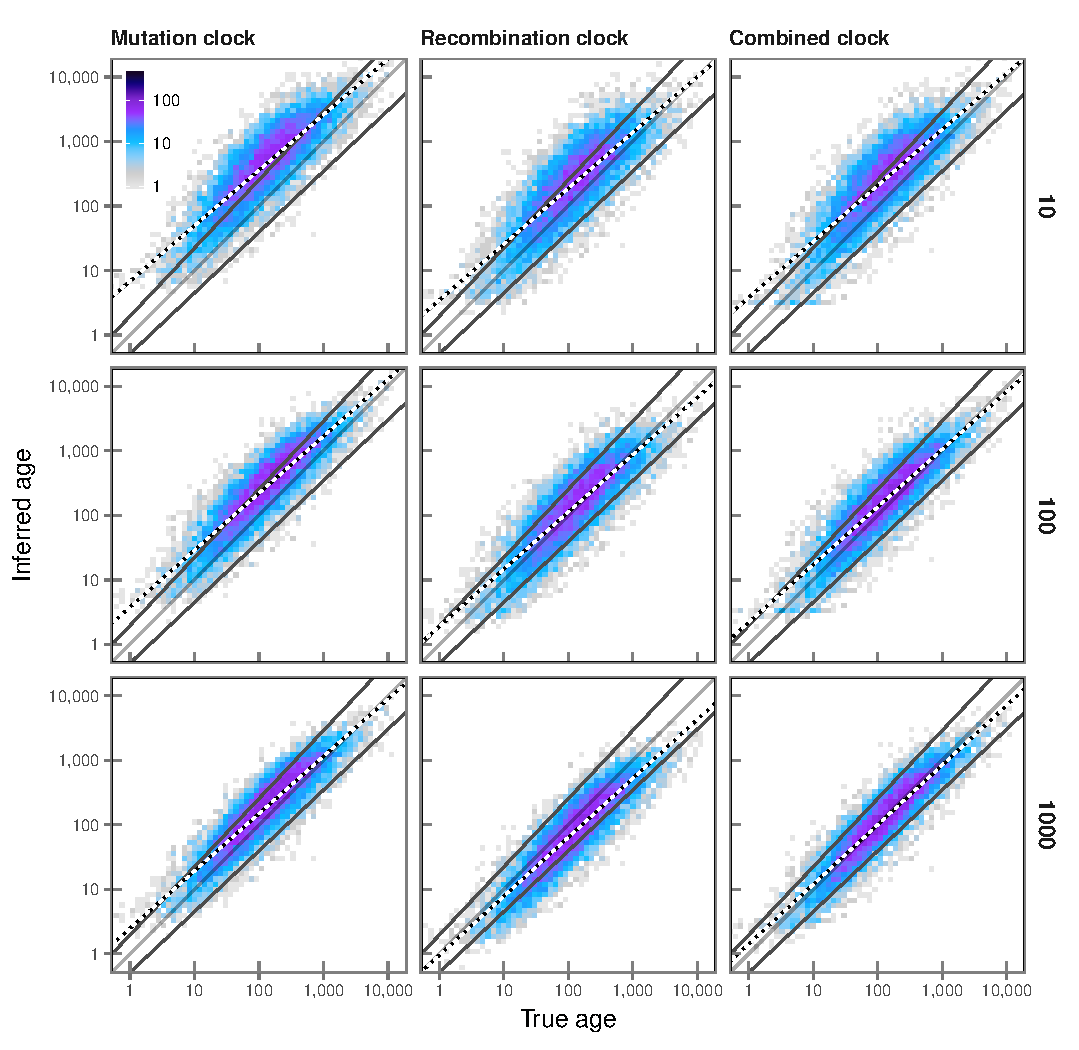
\includegraphics[width=\textwidth]{./img/ch5/discords_scat}
\Caption{True and inferred age under varying numbers of discordant pairs}
{A set of \n{10000} target sites was randomly drawn in \fk{[2,20]} (shared allele frequency ${\leq 1\%}$) in a simulated sample of \n{2000}~haplotypes.
Different numbers of sampled discordant pairs were analysed on the same set of target variants, which is shown for ${n_d = \num{10}}$, ${n_d = \num{100}}$, and ${n_d = \num{1000}}$ (indicated at the \emph{right} of each row).
True IBD was used to estimate allele age.
IBD breakpoints were determined from simulation records and defined as the first variant sites observed in the data following the \n{2} recombination events on each side of a given focal position.
Age was estimated under each of the \n{3} clock models; \ie mutation clock, \ClockM, recombination clock, \ClockR, and combined clock, \ClockC (indicated at the \emph{top} of each column).
Each panel shows the density distribution of true and inferred age (numbers indicated by the colour-gradient).
Note that the ``true age'' of a focal allele was set to $t_m$, which is the geometric mean of $t_c$ and $t_d$, \ie the true time of the coalescent event from which the focal allele derived ($t_c$) and the true time of the coalescent event immediately preceding that event ($t_d$) in the history of the sample, respectively; these are indicated by their regression trend lines \emph{below} and \emph{above} the dividing line at $t_m$, respectively.
The \emph{black-white} line indicates the line of best fit resulting from linear regression of age estimates, using the posterior mode of the composite likelihood distribution as the inferred age value.
True and inferred age are both shown on log-scale.}
{fig:discords_scat}
\end{figure}

%

Despite the substantial difference in the number of pairwise analyses, overall accuracy was high for each threshold and under each clock model.
A higher $n_d$ threshold was generally found to improve overall accuracy.
At lower thresholds, each model showed a tendency to overestimate allele age, which most likely resulted from the smaller set of discordant pairs, as the individuals that are more closely related to the focal haplotypes may or may not be captured.

Interestingly, the recombination clock, \ClockR, showed a tendency to underestimate allele age at higher thresholds, despite using true IBD segments.
This observation may be the result of an overestimation of true IBD lengths, since IBD breakpoints were determined from the set of variant sites observed in the data, to provide a realistic benchmark for comparisons with IBD detection methods (see next section).
Note that allele age is generally expected to be underestimated if genetic lengths in concordant or discordant pairs are overestimated, as a longer IBD segment is indicative for more recent haplotype sharing (\ie recombination had less time the break down the length of a shared haplotype).
The average distance between consecutive variant sites in ${\mathcal{D}_A}$ was \SI{3.064307e-04}{\centi\morgan} (\dec{306.4307} basepairs), showing that even small inaccuracies in IBD can affect the estimation of allele age (under the recombination clock).

The proportion of target alleles for which age was correctly estimated increased with higher $n_d$ thresholds under each clock model.
This was lowest in \ClockM, where \SIlist{36.61;51.11;66.28}{\percent} were correctly inferred for $n_d$ at \numlist{10;100;1000}, respectively, and relatively high in \ClockR, where \SIlist{55.79;70.60;70.51}{\percent} were correct, respectively.
The highest proportion of correct alleles was \SI{79.93}{\percent} in \ClockC and ${n_d = \num{1000}}$.
The proportion of overestimated alleles (${\hat{t} > t_d}$) decreased in all clock models at higher $n_d$ thresholds, showing a modest decrease in \ClockM (\SIrange{63.38}{32.66}{\percent} for $n_d$ at \num{10} and \num{1000}, respectively), a substantial decrease in \ClockR (\SIrange{43.45}{6.45}{\percent}, respectively), and a notable decrease in \ClockC (\SIrange{46.78}{15.64}{\percent}, respectively).
Since \ClockM showed a tendency to overestimate allele age, the proportion of underestimated alleles was low (\SI{1.06}{\percent} for ${n_d = \num{1000}}$), which was similarly low in \ClockC (\SI{4.43}{\percent}), and highest in \ClockR (\SI{23.04}{\percent}).

%
% !TEX root = ../../main.tex


\begin{table}[!htb]
\Caption{Estimation accuracy under varying numbers of discordant pairs}
{Different thresholds for the number of randomly formed discordant pairs, $n_d$, were analysed to evaluate the impact on the accuracy of allele age estimation.
Note that all possible concordant pairs were included in each analysis; \ie $n_c$ was not reduced.
True IBD segments were used to focus on the differences induced by varying $n_d$ thresholds.
Each analysis was conducted on the same set of \n{10000} randomly selected rare variants at allele frequency ${\leq 1\%}$.
Accuracy was measured using the rank correlation coefficient, $r_S$, and the magnitude of error, \gls{rmsle}, between the estimated age, $\hat{t}$ and the times of coalescent events; \ie the time until all haplotypes in $X_c$ have coalesced, $t_c$, and the time of the immediately preceding coalescent event, $t_d$, which joined the lineages in $X_c$ and $X_d$ back in time, as well as the geometric mean of both, $t_m$.}
{tab:stats_discords}
\centering
\begin{tabular}{cS[table-format=4.0]*6{S[table-format=1.3]}}
\toprule
Clock & {$n_d$} &
\multicolumn{3}{c}{Rank correlation ($r_S$)} &
\multicolumn{3}{c}{RMSLE} \\
\cmidrule(lr){3-5}
\cmidrule(lr){6-8}
& & {$t_c$} & {$t_m$} & {$t_d$} & {$t_c$} & {$t_m$} & {$t_d$} \\
\otoprule
\ClockM &   10 &  \bfseries 0.906586 & 0.841847 & 0.631996  &  0.963342 & 0.624464 & \bfseries 0.574325  \\
        &   50 &  \bfseries 0.917657 & 0.872463 & 0.673891  &  0.822642 & \bfseries 0.487039 & 0.528283  \\
				&  100 &  \bfseries 0.920115 & 0.884083 & 0.691649  &  0.763483 & \bfseries 0.430784 & 0.520895  \\
				&  500 &  \bfseries 0.920473 & 0.907259 & 0.731354  &  0.626427 & \bfseries 0.307910 & 0.532824  \\
        & 1000 &  \bfseries 0.923028 & 0.903750 & 0.723312  &  0.606076 & \bfseries 0.298997 & 0.546518  \\
\cmidrule(lr){1-8}
\ClockR &   10 &  \bfseries 0.880780 & 0.816412 & 0.611626  &  0.713779 & \bfseries 0.443323 & 0.609265  \\
        &   50 &  \bfseries 0.889130 & 0.844188 & 0.651051  &  0.577769 & \bfseries 0.348789 & 0.632959  \\
				&  100 &  \bfseries 0.891502 & 0.857111 & 0.670861  &  0.519295 & \bfseries 0.319204 & 0.653344  \\
				&  500 &  \bfseries 0.892486 & 0.886261 & 0.720450  &  0.389722 & \bfseries 0.304215 & 0.727680  \\
        & 1000 &  0.888794 & \bfseries 0.895266 & 0.739364  &  0.345374 & \bfseries 0.329462 & 0.771701  \\
\cmidrule(lr){1-8}
\ClockC &   10 &  \bfseries 0.891099 & 0.829456 & 0.624189  &  0.744861 & \bfseries 0.454964 & 0.589177  \\
        &   50 &  \bfseries 0.900952 & 0.864680 & 0.674755  &  0.623765 & \bfseries 0.348042 & 0.585587  \\
				&  100 &  \bfseries 0.904779 & 0.880661 & 0.698733  &  0.574372 & \bfseries 0.308885 & 0.592973  \\
				&  500 &  0.909421 & \bfseries 0.914094 & 0.752866  &  0.468624 & \bfseries 0.243173 & 0.625955  \\
        & 1000 &  0.910884 & \bfseries 0.913763 & 0.751308  &  0.464245 & \bfseries 0.243365 & 0.629365  \\
\bottomrule
\end{tabular}
\end{table}

%

A complete summary of results is given in \cpref{tab:stats_discords}.
Throughout, rank correlation ($r_S$) was highest for ${n_d = \num{1000}}$; see \cref{tab:stats_discords}.
However, for all thresholds, correlations with $t_c$ were higher than correlations with $t_m$, which in turn were higher than correlations with $t_d$.
Such a pattern may be expected as the number of concordant pairs, $n_c$, was not reduced, such that the $t_c$ was inferred with higher accuracy.
Highest accuracy was seen for the mutation clock model, \ClockM, where $r_S$ for ${n_d = \num{1000}}$ was \dec{0.923028}, \dec{0.903750}, and \dec{0.723312} for $t_c$, $t_m$, and $t_d$, respectively.
By comparison, the recombination clock, \ClockR, yielded the lowest levels of overall accuracy at each threshold, but did not differ markedly from \ClockM; \eg $r_S$ for ${n_d = \num{1000}}$ was \dec{0.888794}, \dec{0.895266}, and \dec{0.739364} for $t_c$, $t_m$, and $t_d$, respectively.
The combined clock, \ClockC, was found to be more accurate for $t_m$ and $t_d$ at higher thresholds.
The magnitude of error, measured by \gls{rmsle} scores, was lowest for $t_m$, indicating that the majority of alleles were correctly dated between $t_c$ and $t_d$; except in \ClockM for ${n_d = \num{10}}$, in which allele age was overestimated and therefore closer to $t_d$.

The difference between ${n_d = \num{500}}$ and ${n_d = \num{1000}}$ was small overall (see \cref{tab:stats_discords}), suggesting that further improvements in accuracy may not be attained by increasing the threshold.

%
% !TEX root = ../../main.tex


\begin{figure}[!htb]
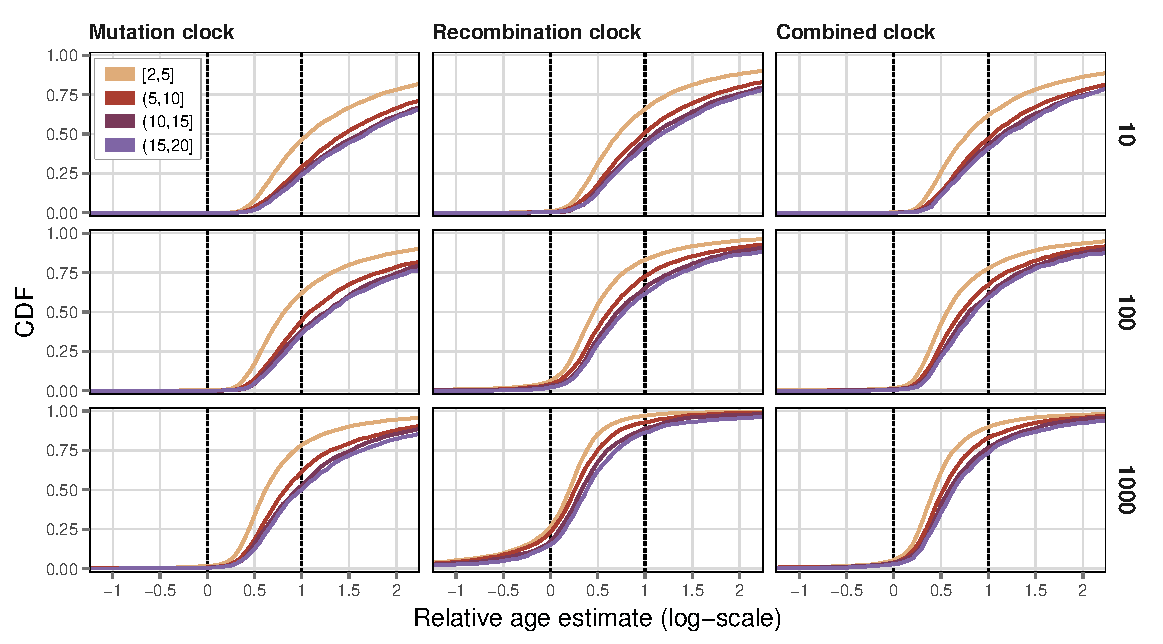
\includegraphics[width=\textwidth]{./img/ch5/discords_hist}
\Caption{Relative age under varying numbers of discordant pairs}
{A randomly drawn set of \n{10000} target sites at allele frequency ${\leq 1\%}$, \ie \fk{[2,20]}, was analysed under each of the \n{3} clock models (indicated at the \emph{top} of each column) and with different numbers of sampled discordant pairs; ${n_d = \num{10}}$, ${n_d = \num{100}}$, and ${n_d = \num{1000}}$ (indicated at the \emph{right} of each row).
The analysis was conducted using the true IBD breakpoints as derived from simulation records, defined as the first variant sites observed in the data that immediately follow the \n{2} recombination events on each side distal to a given focal site.
The relative age, ${\hat{t}_\textit{rel}}$, was calculated as given in \cref{eq:age_relative}, such that the true times of concordant and discordant coalescent events, $t_c$ and $t_d$, sit at 0~and~1, respectively (\emph{dashed} lines).
Note that ${\hat{t}_\textit{rel}}$ is defined on log-scale.
The \gls{cdf} of relative age estimates is shown per \fk{}~group, where target variants were pooled by their allele count in the data, in ranges of \fk{[2,5]}, \fk{(5,10]}, \fk{(10,15]}, and \fk{(15,20]}.}
{fig:discords_hist}
\end{figure}

%

A comparison of the inferred age distributions at distinct \fk{}~ranges is presented in \cpref{fig:discords_hist}, again shown for ${n_d = \num{10}}$, ${n_d = \num{100}}$, and ${n_d = \num{1000}}$.
Notably, the accuracy of target alleles at lower frequencies was overall higher compared to alleles observed at higher frequencies.
This difference was consistent across $n_d$ thresholds under the mutation clock model, \ClockM.
For example, at ${n_d = \num{10}}$, the proportion of correctly dated alleles was higher in the \fk{[2,5]} range (\SI{48.35577}{\percent}) compared to alleles at \fk{(5,10]} (\SI{29.44512}{\percent}).
At ${n_d = \num{1000}}$, overall accuracy was increased but the difference for alleles at lower and higher frequencies remained; \ie \SIlist{77.81947;60.83435}{\percent} at \fk{[2,5]} and \fk{(5,10]}, respectively.
Under the recombination clock model, \ClockR, these differences were reduced at higher $n_d$ thresholds.
At ${n_d = \num{10}}$, \SIlist{66.60781;50.34427}{\percent} of alleles were correctly dated at \fk{[2,5]} and \fk{(5,10]}, respectively, whereas at ${n_d = \num{1000}}$ these proportions were \SIlist{72.25778;69.82584}{\percent} at the same frequency ranges, respectively.

% To explain this observation, consider the genealogical relationship of the sample that is distinguished into $X_c$ and $X_d$ dependent on sharing and non-sharing of a given focal allele, respectively.
% If the focal allele frequency is low, the number of coalescent events that precede the focal mutation event is larger compared to a focal allele shared at a higher frequency in the sample.
% Therefore, a higher $n_d$ threshold increases the chance to randomly

In summary, these results demonstrate that the method as well as the clock models proposed are able to estimate allele age from IBD information alone, without prior knowledge of the demographic history of the sample.
However, because data were simulated under a simple demographic model (dataset $\mathcal{D}_A$), further evaluation is appropriate (\eg using datasets $\mathcal{D}_B$ and $\mathcal{D}_B^{\ast}$; see further below).
The analysis considered true IBD segments and therefore evaded the effects that would result from inexact IBD detection.
Since true IBD was determined conditional on the observed variation in the data, the analysis reflected the practical feasibility of age estimation given available data.


The implemented sampling process seeks to find a compromise between computational tractability and the chance of randomly selecting haplotypes that are informative for the estimation.
However, ideally, to minimise the computational burden while simultaneously improving estimation accuracy, it would be desirable to consider the nearest neighbours to the focal shared haplotypes in the local genealogy.
If the nearest neighbours are found among the haplotypes in $X_d$ and paired with the focal haplotypes in $X_c$ they are likely to coalesce at $t_d$ and are therefore most informative for the estimation of focal allele age.
For instance, a simple approach would be to compute the Hamming distance between haplotypes in $X_c$ and $X_d$ within a short region around the position of a given target site, such that a subset of presumed nearest neighbours can be selected based on a distance ranking.
In practice, however, there are \n{3} caveats to such an approach.

First, it would be computationally expensive to conduct an additional pairwise analysis for the (whole) sample at each target site, which may not outweigh the improvement gained through the reduction of $n_d$.
Second, the identification of nearest neighbours may be less accurate if only genotype data are available.
Both the \gls{dgt} and the \gls{hmm}-based approach implemented in \texttt{rvage} are able to infer IBD in absence of haplotype information; thus, a method to identify nearest neighbours in genotype data would be required to achieve full compatibility with the algorithm.
Regardless, third, a dilemma arises in presence of genotype error, as the identification of nearest neighbours is likely to give preference to haplotypes in which the focal allele has been missed.
\label{p:falseneg}%
Such \emph{false negatives} distort the estimation of allele age as the \gls{ccf}
computed for false discordant pairs would bias (or cancel out) the resulting composite likelihood distribution.
In such cases, the estimated age is expected to be approximately equal to or smaller than $t_c$, such that $\hat{t}$ is likely to be underestimated.

It is important to note that the problem of finding false negatives in the data (if genotype error is present) cannot be avoided if discordant pairs are formed by a random sampling process, but the chance of including false negatives is reduced if $n_d$ is small in comparison to the (haploid) sample size.
Hence, the $n_d$ threshold defines a balance between accuracy and expected bias.
Subsequent analyses were conducted using a threshold equal to the diploid sample size, $N$; that is ${n_d = \num{1000}}$ in analyses using $\mathcal{D}_A$, and ${n_d = \num{2500}}$ using $\mathcal{D}_B$ or $\mathcal{D}_B^{\ast}$.
Since the results presented in this section were obtained on true IBD information, they serve as a benchmark against which different IBD detection methods are compared in the section below.


%
\subsection{Comparison of IBD detection methods}
%

The \texttt{tidy} algorithm for targeted IBD detection (see Chapters~3 and 4) was fully integrated in \texttt{rvage}, such that the \gls{fgt}, \gls{dgt}, and the \gls{hmm}-based approach were available for the inference of IBD segments around focal variants.
Note that genotype data are sufficient for IBD detection using the \gls{dgt} and \gls{hmm}, but haplotypes are required for estimation under the mutation clock model; \ie to count pairwise differences, $S$, along haplotype sequences.
Thus, analyses were conducted on the simulated haplotype dataset ($\mathcal{D}_A$), but haplotype phase was ignored during IBD detection in the \gls{dgt} and \gls{hmm}.
The parameters required by the \texttt{rvage} algorithm were specified accordingly with simulation parameters (${\Ne = \num{10000}}$; ${\mu = \num{1e-08}}$ per site per generation; ${\rho = \num{1e-08}}$ per site per generation).
Here, because simulated data did not include genotype error, theoretical emission model was used in the \gls{hmm}.

The results presented in this section were obtained on the previously selected \n{10000} rare allele target sites, which were analysed using each of the \n{3} IBD detection methods and under each clock model, resulting in a total of \dec{93.295215}~million pairwise analyses.
The fraction of conflicting age estimates differed by clock model as well as IBD detection method; no conflicting estimates were returned when true IBD was used.
Under the mutation clock, \ClockM, analyses using the \gls{fgt} returned \SI{1.808575}{\percent} conflicts.
This fraction was higher using the \gls{dgt} and \gls{hmm}, with \SIlist{2.601097;2.326762}{\percent}, respectively.
Conflicts were seen less under the recombination clock, \ClockR, where none were returned using the \gls{fgt}, but \SIlist{0.010160;0.030481}{\percent} using the \gls{dgt} and \gls{hmm}.
The fraction under the combined clock, \ClockC, was smaller compared to \ClockM, with
\SIlist{1.097337;2.265799;1.818736}{\percent} of conflicted sites using the \gls{fgt}, \gls{dgt}, and \gls{hmm}, respectively.
The remaining sites were intersected to compare clock models and IBD methods on the same set of target sites, retaining \n{9434} variants.

%
% !TEX root = ../../main.tex


\begin{figure}[!htb]
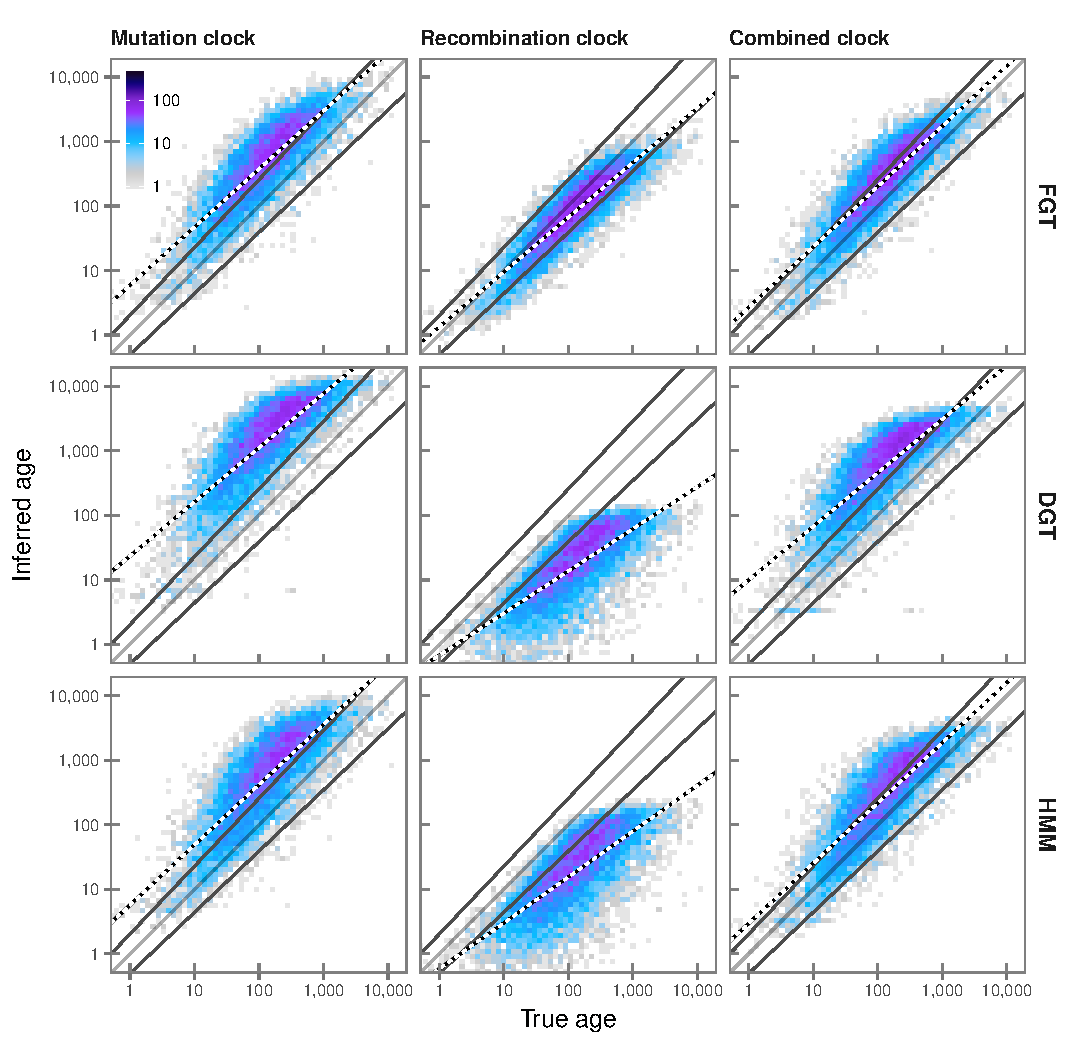
\includegraphics[width=\textwidth]{./img/ch5/vanilla_scat}
\Caption{Distribution of true and inferred age using different IBD detection methods}
{The \n{3} IBD detection methods \gls{fgt}, \gls{dgt}, and \gls{hmm} were compared under each clock model, on the same set of target sites that were drawn from \fk{[2,20]} variants (allele frequency ${\leq 1\%}$) in $\mathcal{D}_A$.
Each panel shows the density of true age ($t_m$) and inferred age.
Lines \emph{below} and \emph{above} the dividing line are regression trend lines of the corresponding true coalescent times around each mutation event, $t_c$ and $t_d$, respectively.
The regression of inferred age ($\hat{t}$) is given by the \emph{black-white} line.}
{fig:vanilla_scat}
\end{figure}

%

The density distribution of true and inferred allele age is given in \cpref{fig:vanilla_scat}.
In all \n{3} methods, a tendency to overestimate allele age was seen, in particular under the mutation clock, \ClockM.
This overestimation was elevated when the \gls{dgt} was used, and less prominent for the \gls{fgt} or \gls{hmm}.
The latter methods showed similar age distributions in \ClockM and under the combined clock model, \ClockC, in which alleles appeared to be less overestimated.
Under the recombination clock, \ClockR, alleles were underestimated in each method, but more severely in both the \gls{dgt} and \gls{hmm}.

Specifically, the method with the highest proportion of correctly estimated alleles was the \gls{fgt} in all \n{3} clock models, where accuracy was highest under the recombination clock, \ClockR, at \SI{72.609710}{\percent}, and lowest under the mutation clock, \ClockM, with \SI{34.46046}{\percent}; under the combined clock, \ClockC, \SI{55.39538}{\percent} of alleles were correctly estimated when the \gls{fgt} was used.
The \gls{hmm} achieved similar levels of accuracy, but the accuracy in \ClockR was noticeably reduced
(\SI{10.949756}{\percent}) compared to \ClockC (\SI{51.87619}{\percent}) and \ClockM \SI{32.41467}{\percent}.
Throughout, the lowest proportions of correctly inferred alleles were found for the \gls{dgt}, which also showed the lowest accuracy in \ClockR (\SIlist{8.225567}{\percent}) and comparatively low levels of accuracy in \ClockM and \ClockC (\SIlist{14.55374;29.65868}{\percent}, respectively).
Overestimation of allele age was highest in \ClockM, where \SIlist{65.08374;85.27666;66.95993}{\percent} of alleles were underestimated by the \gls{fgt}, \gls{dgt}, and \gls{hmm}, respectively.
Conversely, the proportion of underestimated alleles was lowest in \ClockM, at ${\leq 1\%}$ in each method, and similarly low in \ClockC with ${\leq 2\%}$ in each method.
In contrast, alleles were markedly underestimated in \ClockR; the \gls{fgt} resulted in \SI{20.13992}{\percent} of underestimated alleles, whereas \SIlist{91.75323;88.93364}{\percent} of alleles were underestimated when the \gls{dgt} and the \gls{hmm} were used for IBD inference, respectively.

%
% !TEX root = ../../main.tex


\begin{table}[!htb]
\Caption{Estimation accuracy per IBD detection method}
{The accuracy was measured in analyses based on IBD detected by different methods; namely the \gls{fgt}, \gls{dgt}, and the \gls{hmm}-based approach.
See \cpref{tab:stats_discords} for comparison to results obtained using true IBD segments (for ${n_d = \num{1000}}$).}
{tab:stats_vanilla}
\centering
\begin{tabular}{cl*6{S[table-format=1.3]}}
\toprule
Clock & Method &
\multicolumn{3}{c}{Rank correlation ($r_S$)} &
\multicolumn{3}{c}{RMSLE} \\
\cmidrule(lr){3-5}
\cmidrule(lr){6-8}
& & {$t_c$} & {$t_m$} & {$t_d$} & {$t_c$} & {$t_m$} & {$t_d$} \\
\otoprule
\ClockM &  FGT  & \bfseries 0.840676 & \bfseries 0.839366 & \bfseries 0.686220  &  \bfseries 1.011494 & \bfseries 0.652508 & \bfseries 0.554208  \\
        &  DGT  &  0.829831 & 0.812906 & 0.650413  &  1.460099 & 1.085978 & 0.832110  \\
        &  HMM  &  0.805637 & 0.806060 & 0.661580  &  1.077573 & 0.725273 & 0.606789  \\
\cmidrule(lr){1-8}
\ClockR &  FGT  &  \bfseries 0.898918 & \bfseries 0.886870 & \bfseries 0.717613  &  \bfseries 0.338500 & \bfseries 0.329674 & \bfseries 0.774566  \\
        &  DGT  &  0.819520 & 0.749442 & 0.553535  &  0.576894 & 0.940863 & 1.396338  \\
        &  HMM  &  0.820884 & 0.751320 & 0.555899  &  0.532765 & 0.891761 & 1.348435  \\
\cmidrule(lr){1-8}
\ClockC &  FGT  &  \bfseries 0.863498 & \bfseries 0.873015 & \bfseries 0.723484  &  \bfseries 0.754705 & \bfseries 0.422342 & \bfseries 0.523968  \\
        &  DGT  &  0.839769 & 0.828786 & 0.669072  &  1.083494 & 0.726881 & 0.600412  \\
        &  HMM  &  0.825717 & 0.834311 & 0.692021  &  0.806485 & 0.485257 & 0.553758  \\
\bottomrule
\end{tabular}
\end{table}

%

The accuracy measured for each analysis is summarised in \cpref{tab:stats_vanilla}.
The \gls{fgt} under the recombination clock model, \ClockR, showed a higher correlation and slightly reduced error with regard to $t_d$.
There, rank correlation was ${r_S = \dec{0.898918}}$ for the \gls{fgt} and ${r_S = \dec{0.888794}}$ for true IBD; likewise the magnitude of error (\gls{rmsle}) was \dec{0.338500} and \dec{0.345374} for \gls{fgt} and true IBD, respectively.
However, note that a higher accuracy at $t_c$ does not necessarily reflect an improvement in the estimation of actual allele age.
For example, the accuracy with regard to $t_m$ or $t_d$ was lower for the \gls{fgt} compared to true IBD.
In comparison to the other detection methods, the \gls{fgt} outperformed both the \gls{dgt} and \gls{hmm} with regard to each time measure.
The \gls{hmm} showed slightly higher levels of accuracy than the \gls{dgt} in \ClockR, where $r_S$ was higher and \gls{rmsle} lower in terms of each time measure for the \gls{hmm}.
Similarly, in both \ClockM and \ClockC, \gls{rmsle} scores were lower for the \gls{hmm} compared to the \gls{dgt}, whereas $r_S$ measures were similar.

%
% !TEX root = ../../main.tex


\begin{figure}[!htb]
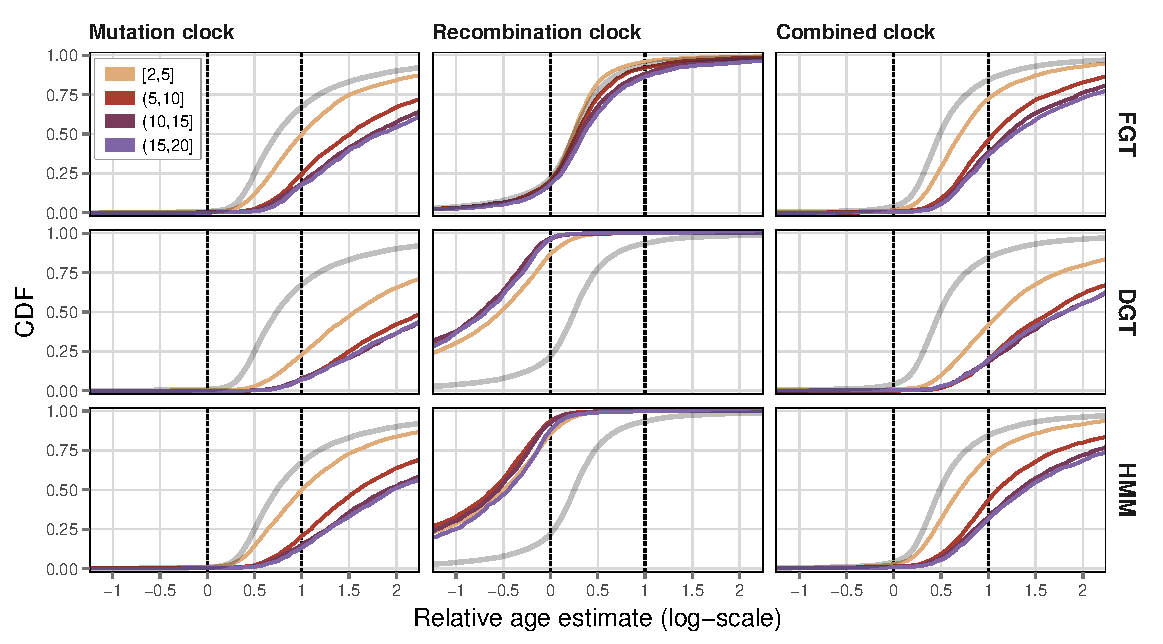
\includegraphics[width=\textwidth]{./img/ch5/vanilla_hist}
\Caption{Relative age using different IBD detection methods}
{The \n{3} IBD detection methods implemented in \texttt{rvage} were compared, \ie \gls{fgt}, \gls{dgt}, and \gls{hmm} (indicated at the \emph{right} of each row), under each clock model (indicated at the \emph{top} of each column).
The relative age, ${\hat{t}_\textit{rel}}$, was calculated as given in \cref{eq:age_relative}, such that $t_c$ and $t_d$ sit at 0~and~1 (\emph{dashed} lines).
The \gls{cdf} of relative age estimates is shown for different frequency ranges; namely \fk{[2,5]}, \fk{(5,10]}, \fk{(10,15]}, and \fk{(15,20]}.
\Correct{The \emph{grey} line provides a comparison to age estimated using true IBD information as shown in \cpref{fig:discords_hist}, but for \fk{[2,20]}.}}
{fig:vanilla_hist}
\end{figure}

%

Relative age estimates are shown for distinct \fk{}~ranges in \cpref{fig:vanilla_hist}, where the relative age of true IBD is indicated for comparison per clock model (calculated on the full \fk{}~range).
Analyses under the mutation clock and the combined clock models, \ClockM and \ClockC, showed a substantial difference between alleles at lower and higher frequencies; \eg overall accuracy of \fk{[2,5]} variants was increased compared to \fk{}~variants at higher frequencies in each method.
This difference was reduced under the recombination clock model, \ClockR, but the \gls{dgt} showed an accuracy decrease for \fk{[2,5]} variants.


%
% !TEX root = ../../main.tex


\begin{figure}[!htb]
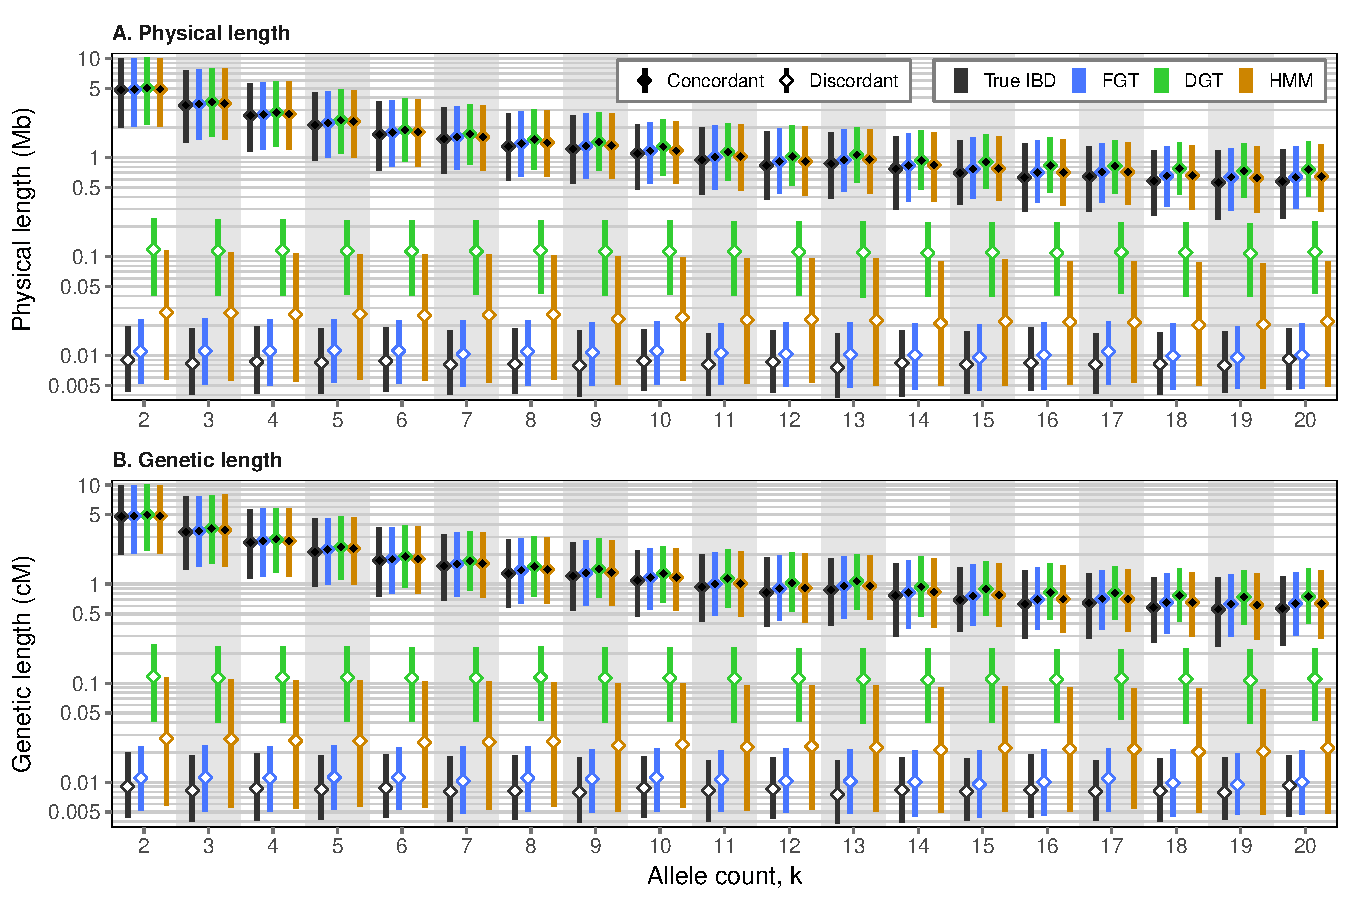
\includegraphics[width=\textwidth]{./img/ch5/vanilla_length_con_dis}
\Caption{Length distribution of inferred IBD segments}
{Bottom and top of each bar indicate \nth{1} and \nth{3} quartiles, respectively, between which the median (\nth{2} quartile) is marked (\emph{diamonds}).
IBD detected for concordant and discordant pairs is distinguished; \emph{solid} and \emph{hollow} diamonds, respectively.}
{fig:vanilla_length_con_dis}
\end{figure}

%

The distribution of IBD lengths inferred using the \gls{fgt}, \gls{dgt}, and the HMM-based approach are shown in \cpref{fig:vanilla_length_con_dis}.
Segments inferred using the HMM were close to those detected using the \gls{fgt} in concordant pairs.
However, for discordant pairs, only the \gls{fgt} produced IBD segments that were close to the length distribution of true IBD segments.
The \gls{dgt} showed the highest degree of overestimation for both concordant and discordant pairs.

In summary, these results suggest that the accuracy of estimated allele age is crucially dependent on correct inference of the underlying IBD structure.
The overestimation of IBD lengths, which is generally expected for each method, affected each clock model differently.
While \ClockM overall resulted in an overestimation of allele age when IBD is overestimated, this pattern was reversed in \ClockR.
Although both models are combined in \ClockC, the impact of mutational differences, seen at the overestimated regions of detected IBD segments, was substantial and could not be mitigated by considering recombinational length.
Further, I confirmed that the \gls{fgt} was the best performing method for the targeted detection of IBD segments, in that the estimation of allele age was similar to the expectations defined by true IBD information.
However, the estimation was more accurate for target sites at lower allele frequencies.
The \gls{dgt} was least accurate in terms of estimated allele age in this comparison.

Recall that the probabilistic model of the \gls{hmm} was developed to overcome the effects of genotype error encountered in real data (see Chapter~4).
Thus, the results in this section reflect theoretical limitations of age estimation given IBD detected in flawless data, but may change drastically in presence of genotype error.
This was explored in the section below.



%
\subsection{Impact of genotype error on allele age estimation}
\label{sec:age_generror}
%

The allele age estimation method was evaluated under each clock model and each method for IBD detection, on data before and after the inclusion of genotype error; \ie using datasets ${\mathcal{D}_B}$ and ${\mathcal{D}_B^{\ast}}$, respectively.
Each analysis was performed on the same set of \n{10000} target sites selected at \fk{[2,25]} in a sample of ${N = \num{2500}}$ diploid individuals, using a threshold of ${n_d = \num{2500}}$, which amounted to \dec{25.281233}~million pairwise analyses per comparison.
The \gls{fgt} was applied to both the simulated (\emph{true}) haplotypes as well as phased haplotype data.
The \gls{hmm} used theoretical emission model in analyses on ${\mathcal{D}_B}$ and the empirical error model in analyses on ${\mathcal{D}_B^{\ast}}$.
To enable direct comparisons, true IBD segments were determined from simulation records and separately analysed on the same number of concordant and discordant pairs in data before and after error.
In total, for the results presented in this section, \dec{758.43699}~million pairwise analyses were conducted.

%
% !TEX root = ../../main.tex


\begin{table}[!htb]
\Caption{Conflicted estimates in analyses before and after error}
{}
{tab:stats_conflicts}
\centering
\begin{threeparttable}
\begin{tabular}{l*6{S[table-format=2.3]}}
\toprule
 Method &
 \multicolumn{3}{c}{Conflicts before error (\%)} &
 \multicolumn{3}{c}{Conflicts after error (\%)} \\
\cmidrule(lr){2-4}
\cmidrule(lr){5-7}
  &  {\ClockM} & {\ClockR} & {\ClockC}  &  {\ClockM} & {\ClockR} & {\ClockC} \\
\otoprule
FGT*       &   6.396224 & 0.000000 & 3.695150  &   5.131037 & 0.140576 & 2.188974 \\
FGT**      &   6.587006 & 0.421729 & 4.387990  &   4.940255 & 0.341399 & 3.122803 \\
DGT        &  10.944874 & 0.160658 & 8.384375  &   5.211366 & 1.767245 & 3.956220 \\
HMM        &   5.884124 & 0.391605 & 4.418114  &  13.334672 & 0.823375 & 9.267998 \\
\cmidrule(lr){1-7}
True IBD   &   0.000000 & 0.000000 & 0.000000  &   9.583101 & 0.000000 & 1.030332 \\
\bottomrule
\end{tabular}
\begin{tablenotes}\footnotesize
	\item[{${\ast}$}] ~ FGT applied to true haplotypes
	\item[{${\ast\ast}$}] ~ FGT applied to phased haplotypes
\end{tablenotes}
\end{threeparttable}
\end{table}

%

As in the previous section, some of the analyses returned conflicting estimates; see \cref{tab:stats_conflicts}.
Again, no conflicts were seen when true IBD information was used.
However, this changed after the inclusion of genotype error; the fraction of conflicting estimates was high in \ClockM, zero in \ClockR, and small in \ClockC.
Before error, the largest fraction of conflicts was seen for the \gls{dgt} in \ClockM.
Data from analyses before and after error were intersected across results obtained under each clock model and for each IBD method, which retained a set of \n{5015} identical target sites.
A complete summary of the accuracy per analysis is given below in \cpref{tab:stats_generror}.

%
% !TEX root = ../../main.tex


\begin{figure}[tb]
{\small\texthv{\textbf{\,(a) True IBD}}} \\
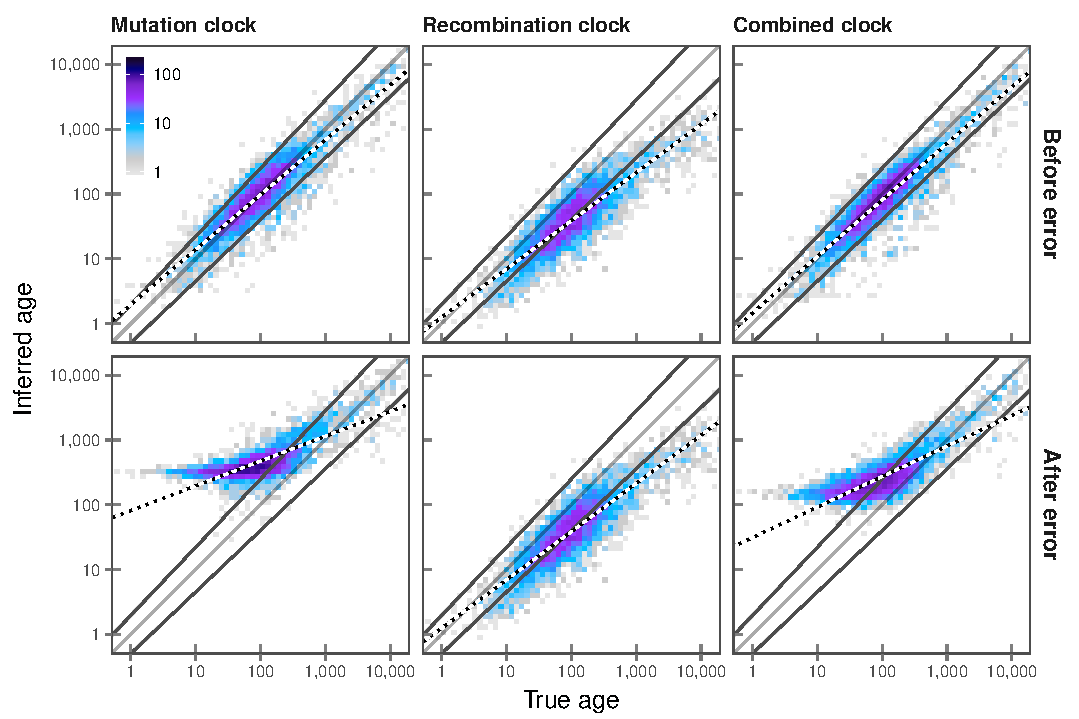
\includegraphics[width=\textwidth]{./img/ch5/generror_scat_tru}
\Caption{Density of allele age before and after error in simulated data}
{The effects on the estimation process \emph{before} and \emph{after} error are compared.
Note that the ``true age'' was set to $t_m$, which is the geometric mean of $t_c$ and $t_d$.
Lines \emph{below} and \emph{above} the dividing line correspond to the regression lines over $t_c$ and $t_d$; \ie of the times of coalescent events delimiting the branch on which a focual mutation occurred.
The \emph{black-white} line gives the regression for the inferred age ($\hat{t}$).
This panel (\textbf{a}) compares the distributions of true and inferred ages, which were estimated on basis of the true IBD structure of the sample as determined from simulation records.
The other panels show estimation results based on the different IBD detection methods;
\gls{fgt} on both true and phased haplotypes (\textbf{b}, \textbf{c}; \pref{fig:generror_scat_fgt}),
\gls{dgt} (\textbf{d}; \pref{fig:generror_scat_dgt}),
and the genotype-based \gls{hmm} (\textbf{e}; \pref{fig:generror_scat_hmm}).
Each analysis was conducted on the same set of \n{5000} randomly selected target variants at \fk{[2,25]}.}
{fig:generror_scat_tru}
\end{figure}

%

Estimation based on the true IBD structure of the sample is compared before and after error in \cref{fig:generror_scat_tru}{a} (\pref{fig:generror_scat_tru}).
The most striking discovery is the extent of overestimation after error under the mutation clock model, \ClockM, which was similarly high in the combined clock, \ClockC.
Alleles were overestimated because the presence of misclassified alleles substantially increased the number of observed mutational differences, $S$, along the sequence.
For example, accuracy decreased in \ClockM from ${r_S = \dec{0.869553}}$ to ${r_S = \dec{0.517705}}$ with regard to $t_c$, before and after error respectively, similarly in \ClockC, where $r_S$ at $t_c$ decreased from \dec{0.884482} to \dec{0.592839}, respectively.
The proportion of correctly estimated alleles (${t_c < \hat{t} < t_d}$) in \ClockM was \SI{75.39382}{\percent} before and \SI{24.06780}{\percent} after error, which was similar in \ClockC, where \SI{80.51844}{\percent} of alleles were correct before but only \SI{39.40179}{\percent} after error.
The proportion of overestimated alleles was
\SI{18.04586}{\percent} in \ClockM and \SI{9.212363}{\percent} in \ClockC before error, but \SI{74.39681}{\percent} and \SI{57.92622}{\percent}, respectively, after error.
Note that this did not vary noticeably by focal allele frequency; for example, the proportion of overestimated alleles in \ClockM was \SI{75.65938}{\percent} at lower frequencies (\fk{[2,5]}) and \SI{79.37500}{\percent} at higher frequencies (\fk{[20,25]}), which was also the case in \ClockC, where \SIlist{61.83120;1.25000}{\percent} of alleles were overestimated at \fk{[2,5]} and \fk{[20,25]}, respectively.

In contrast, the estimation under the recombination clock model, \ClockR, was not affected by genotype error, due to using true IBD information to derive recombinational segment lengths.
Note that analyses were performed on the same sets of concordant and discordant pairs, which is why the results in \ClockR are identical before and after error.
As in the previous analysis, alleles showed a tendency to be underestimated in \ClockR.
The average distance between consecutive \glspl{snp} was \SI{1.609087e-04}{\centi\morgan} (\dec{93.55677} basepairs) in ${\mathcal{D}_B}$ and ${\mathcal{D}_B^{\ast}}$; \ie the density of variant sites is higher compared to ${\mathcal{D}_A}$, such that a potential bias resulting from overestimation of true IBD lengths is expected to be reduced.
Overall, \SI{42.89132}{\percent} of alleles were correctly inferred, but this was higher for at \fk{[2,5]} and lower at \fk{[20,25]}; \SIlist{48.68124;39.37500}{\percent}, respectively.
The proportion of underestimated alleles was \SI{55.55334}{\percent}, where \SIlist{50.52751;52.50000}{\percent} were underestimated at \fk{[2,5]} and \fk{[20,25]}, respectively.
The correlation between inferred and true age was generally high
($r_S$: \numlist{0.818219;0.842606;0.665742} at $t_c$, $t_m$, and $t_d$, respectively)
but nonetheless slightly lower compared to corresponding results from dataset ${\mathcal{D}_A}$
(\numlist{0.888794;0.895266;0.739364}, respectively); although, note that these results are not directly comparable as the underlying demographies were different and only half the number of target sites was analysed here.

%
% !TEX root = ../../main.tex


\begin{figure}[p]
\ContinuedFloat
{\small\texthv{\textbf{\,(b) FGT, true haplotypes}}} \\
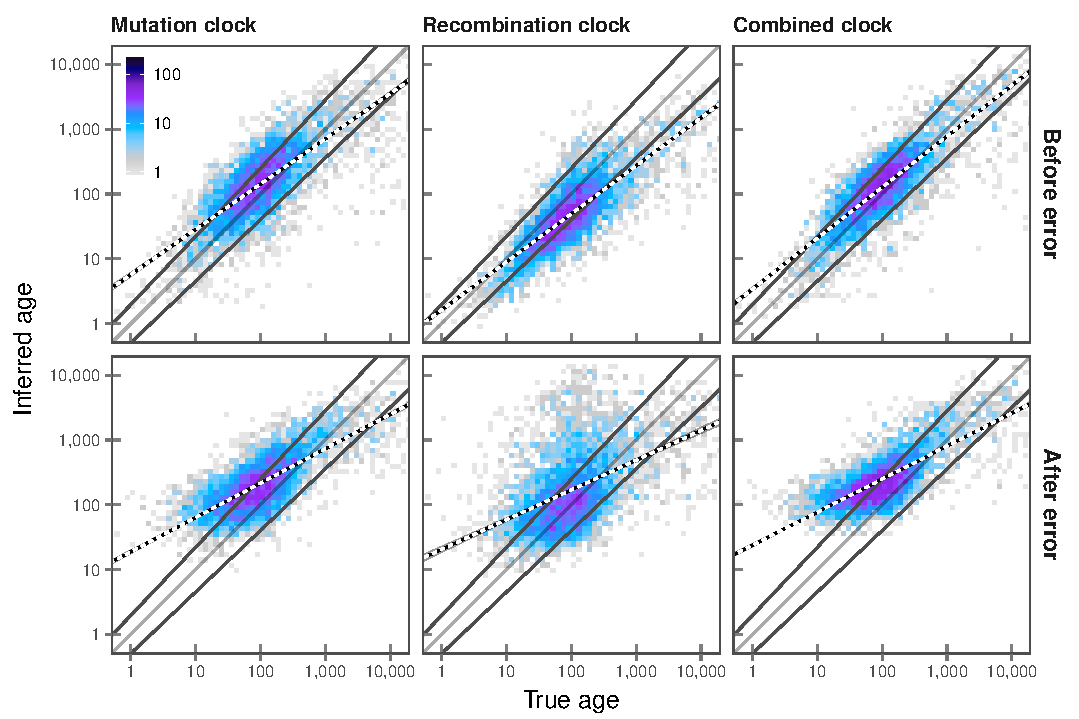
\includegraphics[width=\textwidth]{./img/ch5/generror_scat_fgtH}
{\small\texthv{\textbf{\,(c) FGT, phased haplotypes}}} \\
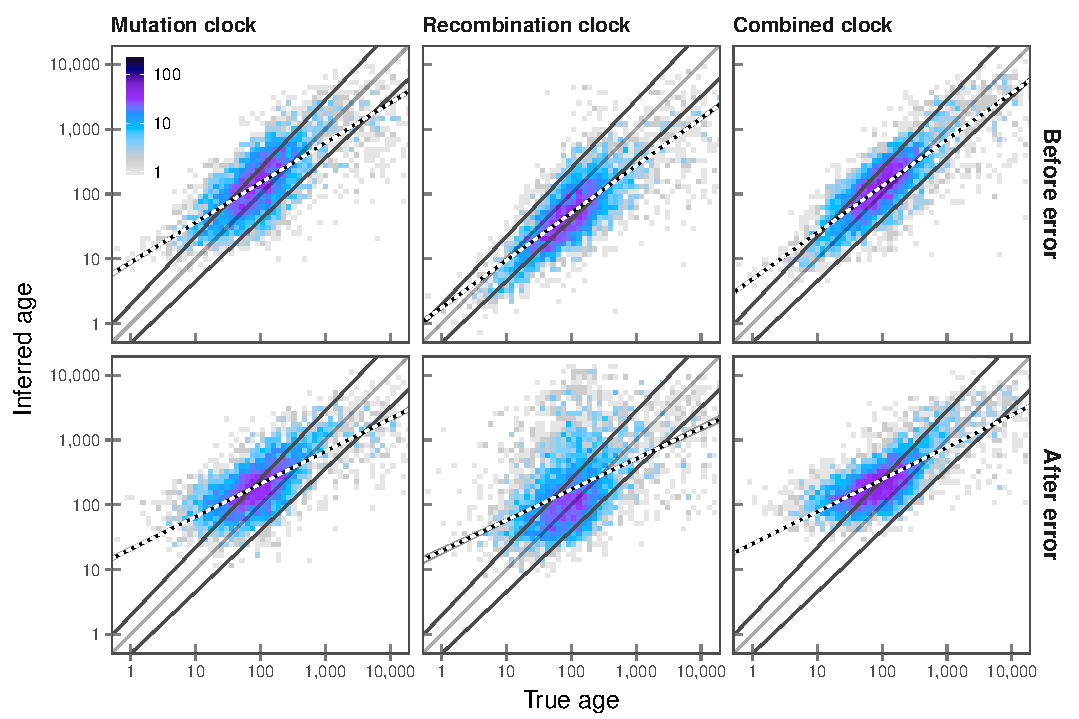
\includegraphics[width=\textwidth]{./img/ch5/generror_scat_fgtP}
\caption[]{Continued.}
\label{fig:generror_scat_fgt}
\end{figure}

%

When IBD was inferred, the accuracy of the estimation analysis was differently affected dependent on the IBD detection method used.
Results based on the \gls{fgt} are shown in
\cref{fig:generror_scat_fgt}{b} and \ref{fig:generror_scat_fgt}{c} (\pref{fig:generror_scat_fgt}), which compare age estimates obtained on the same set of target sites based on IBD detected in true and phased haplotypes, respectively, both before and after error.
Without genotype error, \SIlist{53.02094;50.84745;60.03988}{\percent} of alleles were correctly inferred from true haplotype data in \ClockM, \ClockR, and \ClockC, respectively.
When phased data were used, this changed only slightly; \SIlist{50.82752;51.365902;59.18245}{\percent} of correct alleles in \ClockM, \ClockR, and \ClockC, respectively.
Note that the proportion of correctly inferred alleles increased in \ClockR due to phasing error.
This is because the underestimation that was generally seen under the recombination clock model may have been mitigated by further reduction of IBD segment lengths resulting from flip or switch errors in phased data.
The small difference between true and phased data was further reflected in the accuracy of each analysis, where $r_S$ changed from \numrange{0.679635}{0.660366} in \ClockM, \numrange{0.779995}{0.764215} in \ClockR, and \numrange{0.741871}{0.731383} in \ClockC, with regards to $t_d$.

When analyses were performed on data with genotype error, the overall proportion of correct alleles was reduced, but again the differences seen from true and phased data were small.
On true haplotypes, the proportion of correct alleles was \SIlist{44.26720;45.024925;42.03390}{\percent} in \ClockM, \ClockR, and \ClockC, respectively, whereas \SIlist{43.54935;46.001994;41.63509}{\percent} of alleles were correct using phased haplotypes in \ClockM, \ClockR, and \ClockC, respectively.
Likewise, accuracy was overall reduced but $r_S$ and \gls{rmsle} scores did not suggest notable differences between estimation results from true and phased haplotypes; see \cpref{tab:stats_generror}.
Notably, the analysis on true IBD suggested that genotype error induces an overall overestimation of allele age in \ClockM and \ClockC.
However, this effect was mitigated by underestimating IBD lengths in the \gls{fgt}, such that the number of pairwise differences, $S$, may not be elevated as genotype errors that would increase the value of $S$ may also lead to the premature detection of interval breakpoints.

%
% !TEX root = ../../main.tex


\begin{figure}[tb]
\ContinuedFloat
{\small\texthv{\textbf{\,(d) DGT}}} \\
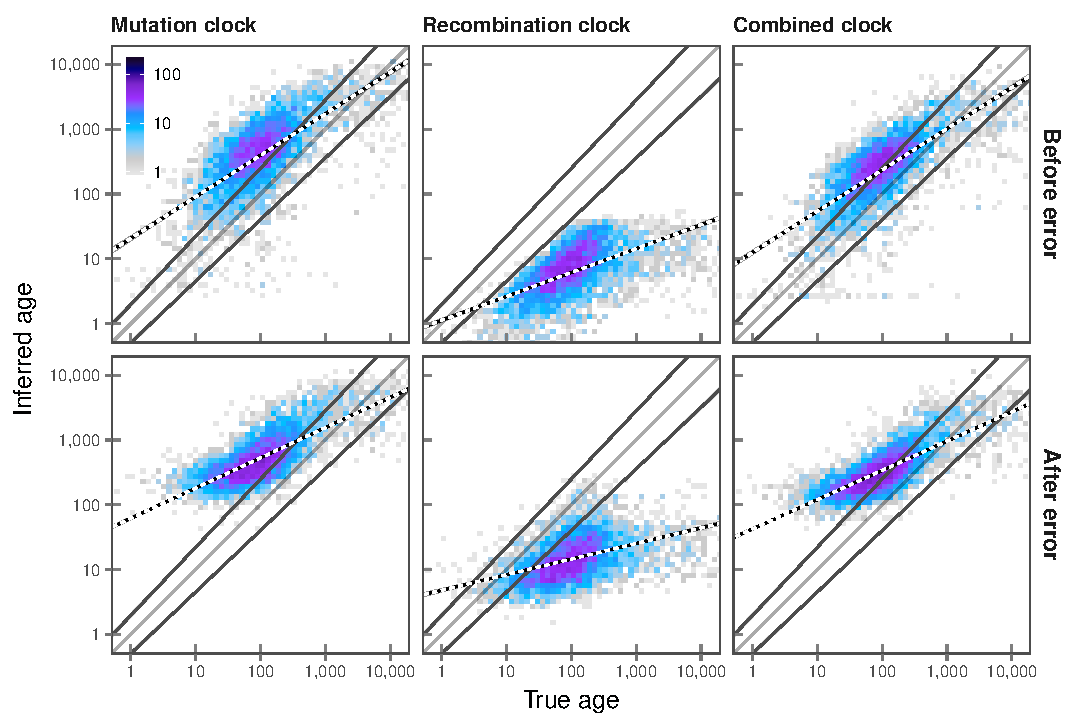
\includegraphics[width=\textwidth]{./img/ch5/generror_scat_dgt}
\caption[]{Continued.}
\label{fig:generror_scat_dgt}
\end{figure}

%

Estimation results based on the \gls{dgt} for IBD detection are shown in \cref{fig:generror_scat_dgt}{d} (\pref{fig:generror_scat_dgt}).
Before error, the proportions of correctly inferred allele age were the lowest in the present comparison in each clock model.
Under both the mutation and combined clocks, \ClockM and \ClockC, \gls{dgt}-based age estimation resulted in \SIlist{26.34098;36.94915}{\percent} of correct alleles, respectively, whereas only \SI{2.412762}{\percent} were correct in \ClockR.
While the majority of alleles in \ClockM and \ClockC were overestimated, \SIlist{70.04985;57.84646}{\percent} respectively, \SI{97.58724}{\percent} were underestimated in \ClockR (none were overestimated).
The tendency to overestimate allele age was increased after error; the proportions of alleles overestimated were \SIlist{77.30808;67.85643}{\percent} in \ClockM and \ClockC, respectively.
As this was also the case in \ClockR, the proportion of correctly inferred alleles increased to \SI{15.692921}{\percent}, but this was an artefact resulting from an overall underestimation of IBD lengths.
However, the loss in accuracy was reflected in the correlation between true and inferred allele age; $r_S$ at $t_c$, $t_m$, and $t_d$ was \numlist{0.746385;0.627943;0.406151} before error, and \numlist{0.588234;0.504469;0.328094} after error.
Note that rank correlations at $t_m$ and $t_d$ were higher in \ClockM and \ClockC, both before and after error.
However, the same measures taken after error actually suggested that the accuracy increased in \ClockM and \ClockC; see \cpref{tab:stats_generror}.
Regardless, rank correlation measured at $t_c$ was decreased after error under each clock model.

%
% !TEX root = ../../main.tex


\begin{figure}[tb]
\ContinuedFloat
{\small\texthv{\textbf{\,(e) HMM}}} \\
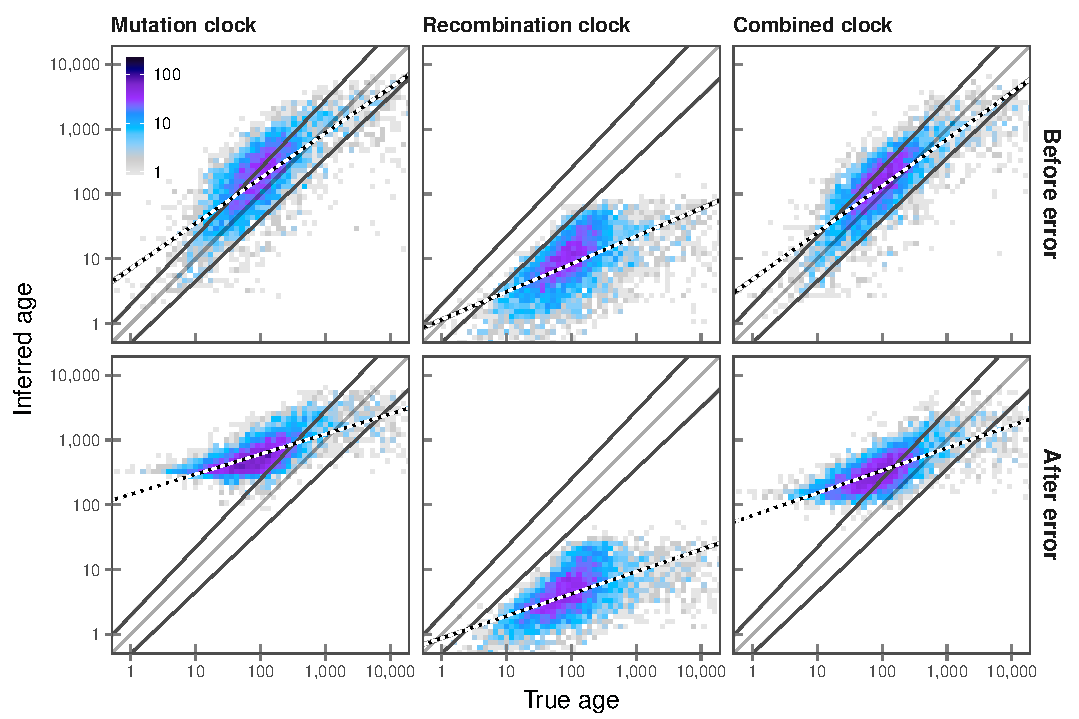
\includegraphics[width=\textwidth]{./img/ch5/generror_scat_hmm}
\caption[]{Continued.}
\label{fig:generror_scat_hmm}
\end{figure}

%

The accuracy of age estimation based on IBD inference using the \gls{hmm}-based approach was overall highly accurate before error; more accurate in comparison to the \gls{fgt} in \ClockM, similar in accuracy to the \gls{dgt} in \ClockR, and similar to the \gls{fgt} in \ClockC.
The density distribution for results obtained using the \gls{hmm} is given in \cref{fig:generror_scat_hmm}{e} (\pref{fig:generror_scat_hmm}).
Before error, the proportion of correct alleles was \SI{47.53739}{\percent} in \ClockM, \SI{3.629113}{\percent} in \ClockR, and \SI{57.82652}{\percent} in \ClockC.
The majority of alleles was underestimated in \ClockR (\SI{96.35095}{\percent}).
This was increased after error, \ie \SI{98.30508}{\percent} in \ClockR, as the proportion of correct alleles was overall reduced; \SIlist{16.65005;27.65703}{\percent} in \ClockM and \ClockC, respectively.
For example, \gls{rmsle} scores were lowest for the \gls{hmm} under each clock model after error; see \cpref{tab:stats_generror}.
The accuracy before and after error, measured as $r_S$ at $t_c$, decreased from \dec{0.702418} to \dec{0.534920} in \ClockM, and from \dec{0.733298} to \dec{0.569244} in \ClockC.
However, importantly, the \gls{hmm}-based estimation showed the highest levels of accuracy in \ClockR compared to the other methods, \ie $r_S$ at $t_c$ was \dec{0.751100} before and \dec{0.737036} after error.
Although allele age was vastly underestimated, deviations appeared to be consistent.

%
% !TEX root = ../../main.tex


\begin{figure}[p]
{\smaller\texthv{\textbf{(a) Before error}}}\\
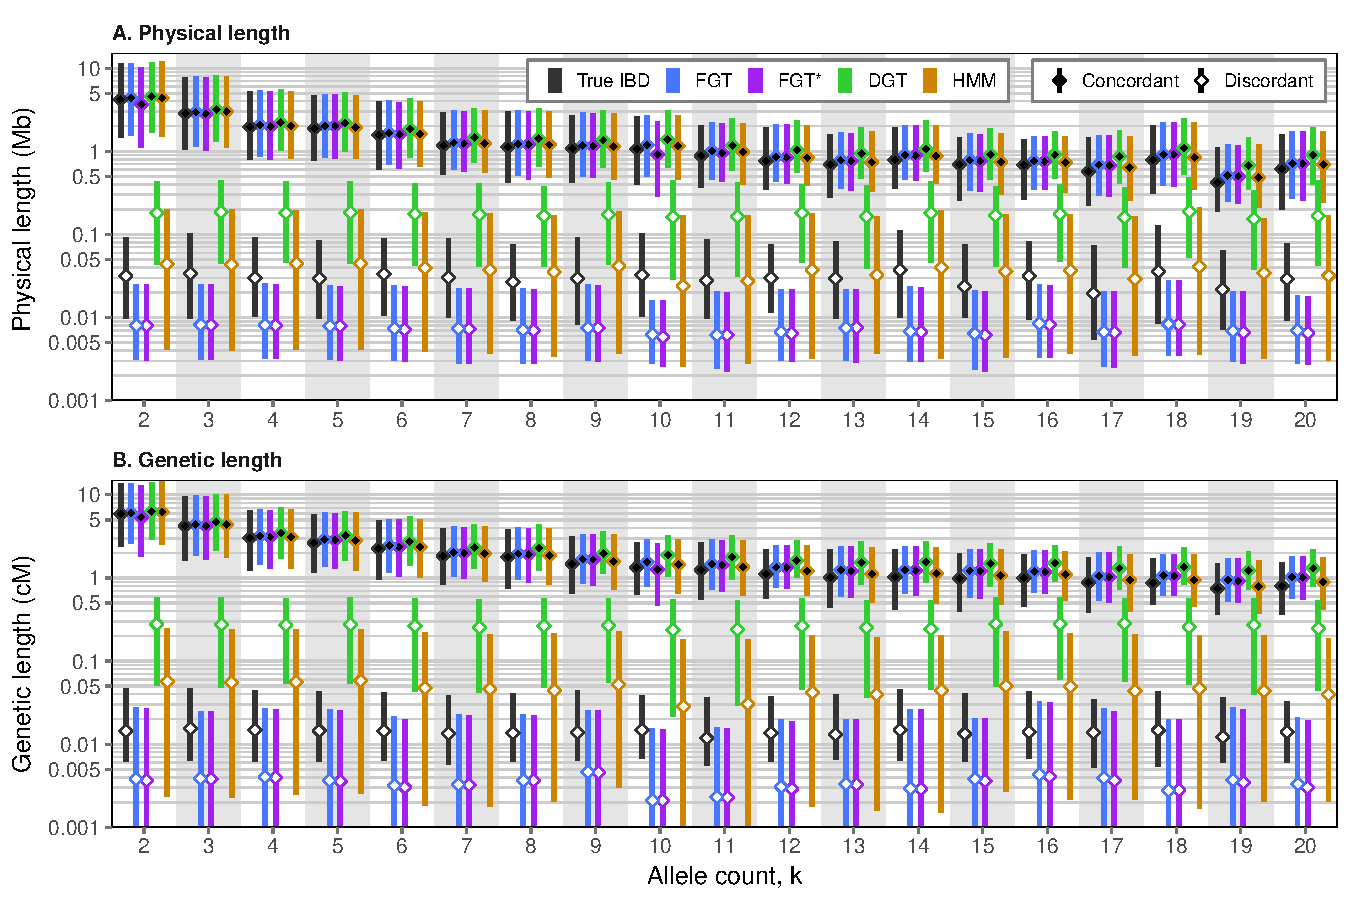
\includegraphics[width=\textwidth]{./img/ch5/africa_length_con_dis_tru}
{\smaller\texthv{\textbf{(b) After error}}}\\
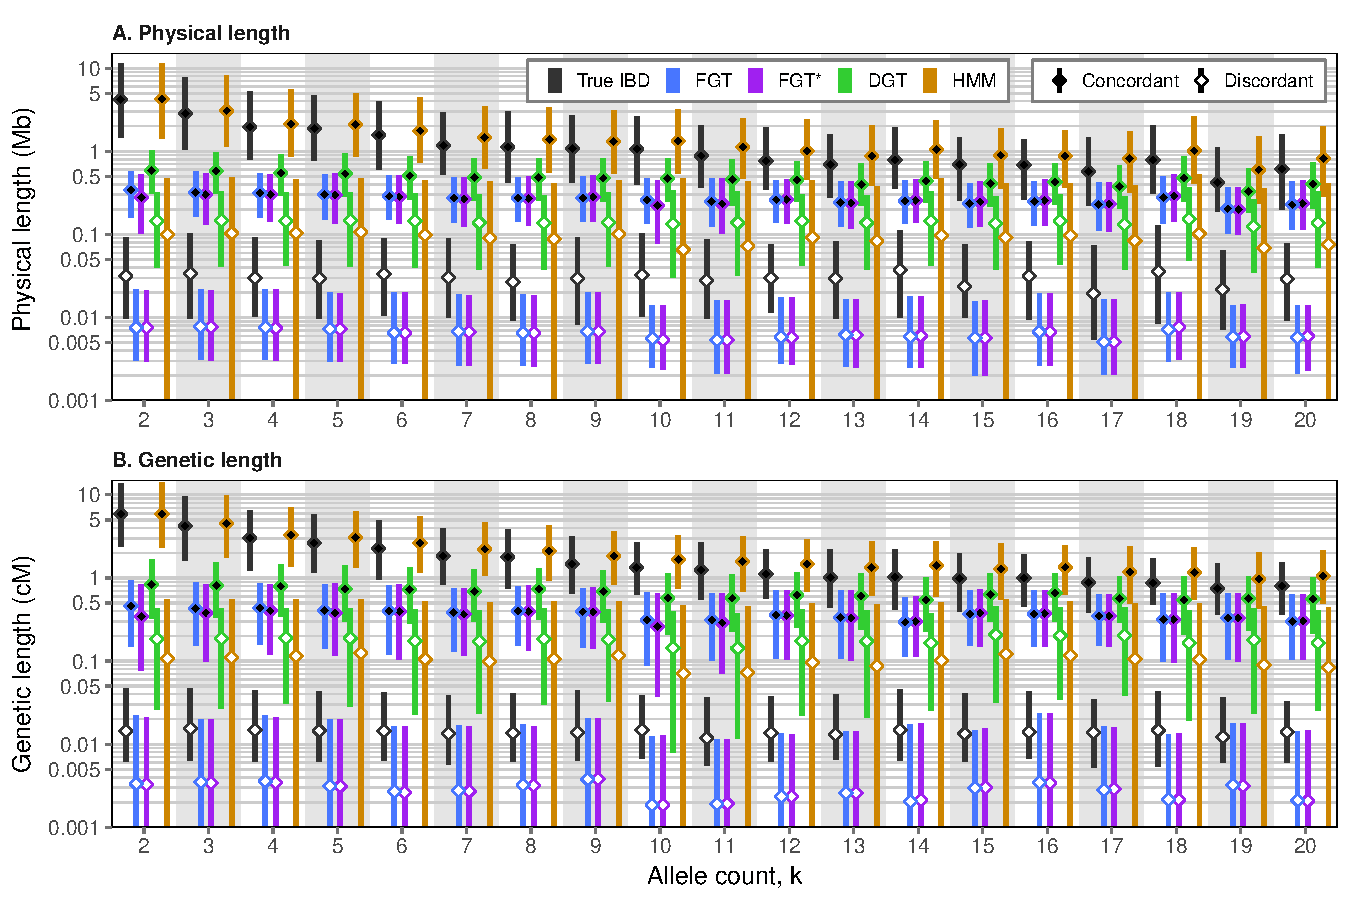
\includegraphics[width=\textwidth]{./img/ch5/africa_length_con_dis_err}
\Caption{Length distribution of inferred IBD segments before and after error}
{Bottom and top of each bar indicate \nth{1} and \nth{3} quartiles, respectively, between which the median (\nth{2} quartile) is marked (\emph{diamonds}).
IBD detected for concordant and discordant pairs is distinguished; \emph{solid} and \emph{hollow} diamonds, respectively.}
{fig:africa_length_con_dis}
\end{figure}

%

The distribution of inferred IBD segment lengths for each approach are given in \cpref{fig:africa_length_con_dis}.
Notably, IBD segments detected using the \gls{fgt} and \gls{dgt} were overall underestimated after error; only the HMM maintained similarly accurate lengths before and after error, for both concordant and discordant pairs.

%
\subsubsection{Generation of error correction models}
\label{sec:age_corrfactor}
%

Although the estimation showed strong tendencies to either over- or underestimate allele age, dependent on the clock model and IBD method used, some settings maintained relatively high levels of accuracy after error; in particular the \gls{hmm}-based inference in \ClockR.
This suggested that deviations from the true age may follow a consistent pattern.
As it is hoped that the age estimation method presented in this chapter is able to produce credible results when used on real data, I evaluated the reliability of each estimation approach by constructing error correction models specific to each setting.

The deviation of the estimated age, $\hat{t}$, from the actual true age of an allele, denoted by $t^\ast$, is simply the absolute value of their difference; calculated as ${\delta = | \hat{t} - t^\ast |}$.
Given the expectation that the time to coalescence is exponentially distributed, the logarithmic difference is calculated as
\begin{equation}
	\xi ~=~ \frac{t^\ast \euler{-\delta}}{\hat{t}}
\end{equation}
where ${\xi = 0}$ if true and estimated age are equal, ${0 < \xi < 1}$ if the age is overestimated, and ${\xi > 1}$ if age is underestimated.
As the actual age of an allele was not known from coalescent simulations, here, the midpoint of the branch on which the mutation event occurred, $t_m$, was defined as the reference point against which the estimated age was compared.
In reverse, a constant $\xi$ value was used as a correction factor applied to a given set of analysed alleles, considering the results obtained per clock model and IBD method, in order to minimise the mean of the difference distribution.
The value of this correction factor was estimated by iteration through an array, denoted by $\Xi$, which is defined as a series of $l$ factor values, denoted by ${\xi_i \in \Xi}$, where ${i \in [ 1, 2, \ldots l]}$.
The minimum factor value was found through the following operation;
\begin{equation}\label{eq:corrfactorcalc}
	i = \argmin_{\xi_i ~\in~ \Xi} \left( \bigg| ~ \frac{1}{n} \sum_{j=1}^n \log \big[ {t_m}_j \big] - \log \big[ \hat{t}_j ~ \xi_i \big] ~ \bigg| \right)
\end{equation}
which is applied to a given set of $n$ true and corresponding estimated times, ${t_m}_j$ and ${\hat{t}_j}$, respectively, where ${j \in 1, 2, \ldots, n}$.
I applied \cref{eq:corrfactorcalc} in a recursive algorithm in which I selected $\xi_{i-1}$ and $\xi_{i+1}$ after each step to redefine the limits of $\Xi$ and to recalculate $l$ new factor values for the next step.
This greatly improved the speed and resolution of the computation.

%
% !TEX root = ../../main.tex


\begin{figure}[!htb]
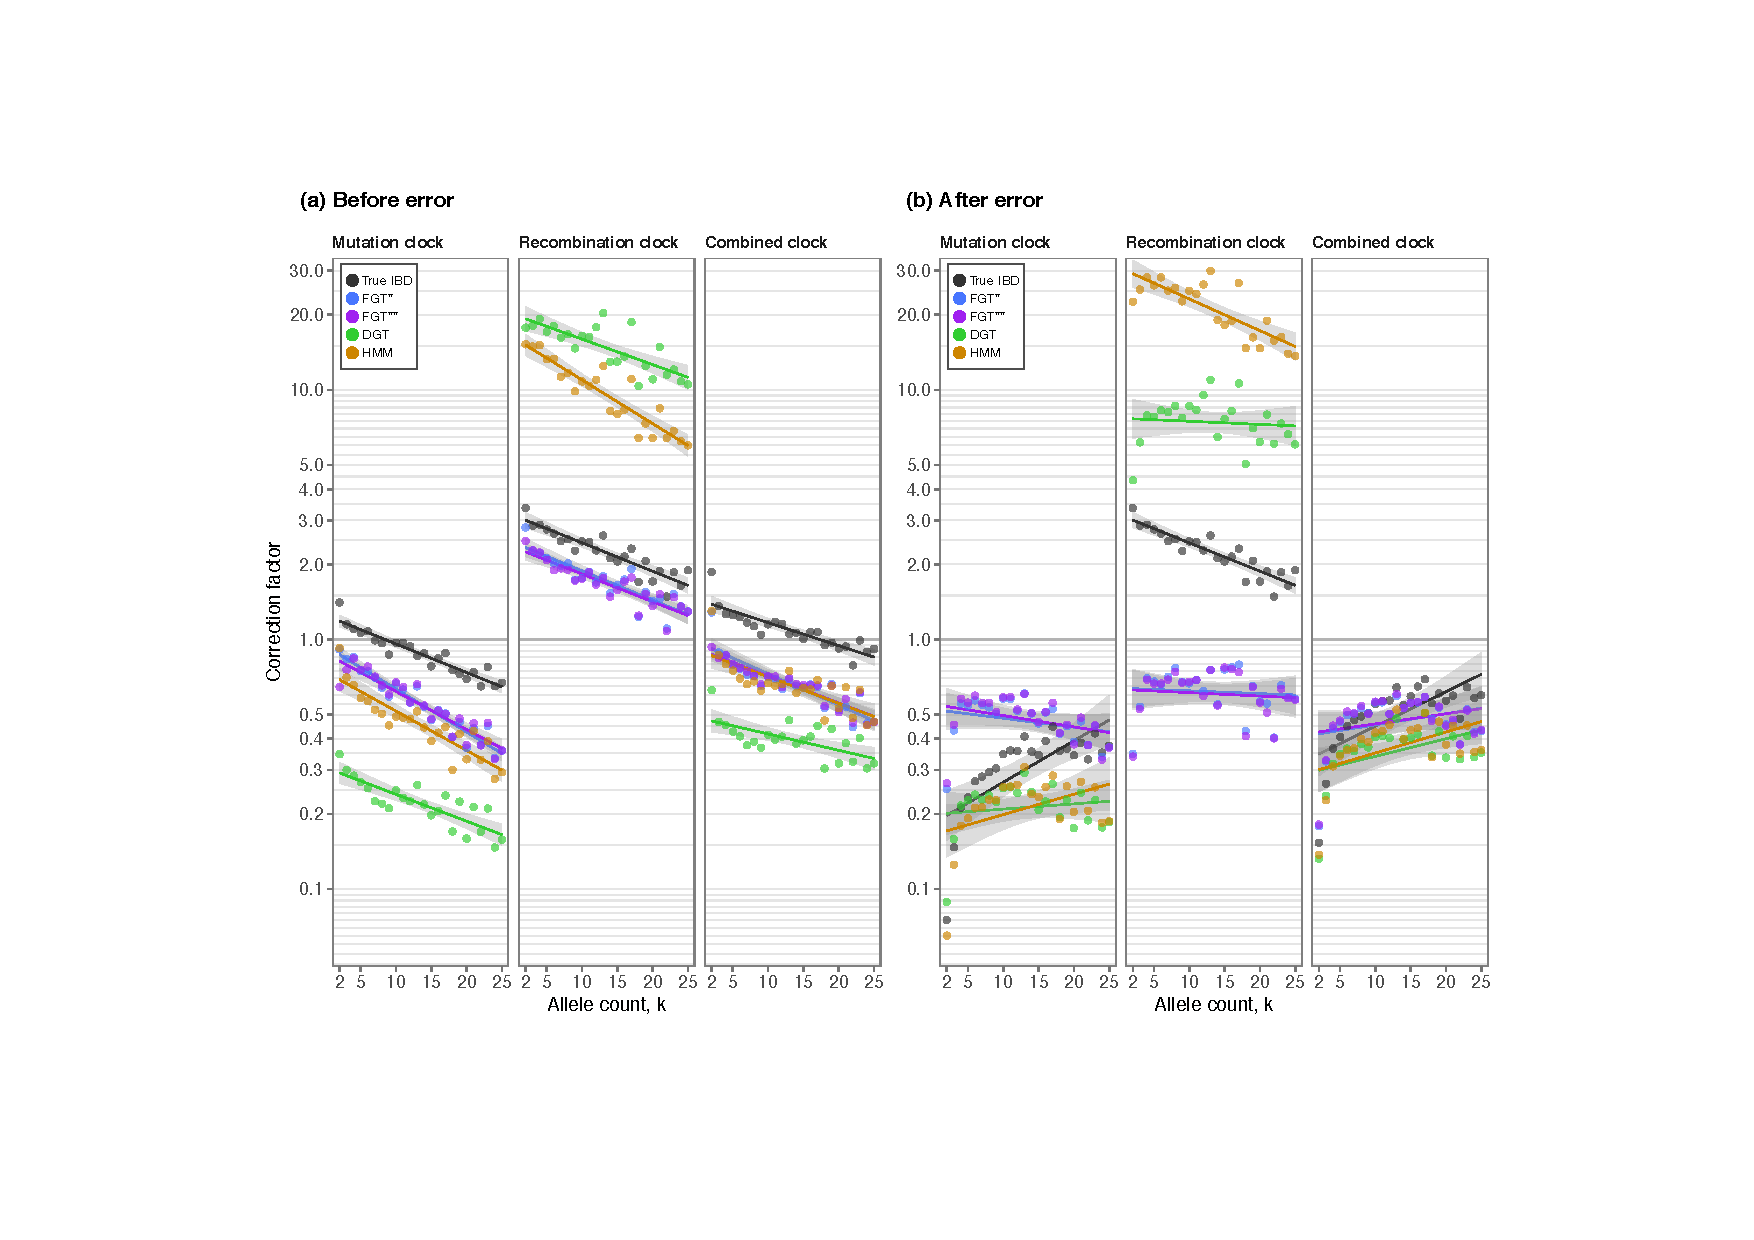
\includegraphics[width=\textwidth]{./img/ch5/generror_factor}
\Caption{Estimated correction factors before and after error}
{Correction factors were estimated per set of \fk{}~variants for which allele age was estimated in each analysis under a given clock model and IBD detection method.
Values below and above 1 indicate that true age was overestimated and underestimated on average, respectively.
The line shown per analysis indicates the trend of the corrected deviation ($\pm\,\text{SE}$), which was calculated through simple nonlinear regression by allele frequency.
Note that IBD detection using the \gls{fgt} was performed on true haplotype data (*) as well as phased haplotypes (**).}
{fig:generror_factor}
\end{figure}

%

The algorithm outlined above was applied on the results obtained per set of \fk{}~variants estimated in each clock model and IBD method, as well as true IBD, before and after error.
Computed correction factors are shown in \cref{fig:generror_factor}, which highlights that deviations followed a general trend in each analysis.
For example, before error, allele age estimated using true IBD showed the lowest amount of deviation in \ClockM and \ClockC, but where alleles at lower frequencies showed a tendency to be overestimated on average and underestimated at higher frequencies.
However, in \ClockR, true IBD showed larger deviations compared to the \gls{fgt} (on both true and phased haplotype data), but this may result from the assumption that $t_m$ approximates the actual age of an allele.
After error, notably, factor deviations showed spurious patterns for most approaches, except for the \gls{hmm}-based estimation of allele age, which indicated a consistent trend.
Note that the factor distributions of true IBD in \ClockR were identical before and after error, as genotype error did not affect the estimation under the recombination clock when IBD is known.

Generated error correction factors were applied to the estimated age results, after error, at corresponding \fk{}~variants under each clock model and in each IBD method, which minimised deviations in relation to $t_m$.
As a consequence, accuracy was overall improved in each approach; see \cpref{tab:stats_generror}.
Notably, however, the rank correlation measured for the \gls{hmm} in \ClockR was least affected; before applying correction factors, $r_S$ was \numlist{0.737036;0.621305;0.397976} at  $t_c$, $t_m$, and $t_d$, respectively, which was marginally improved after correction, yielding \numlist{0.737611;0.624484;0.402304}, respectively.
Nonetheless, the \gls{hmm} indicated the highest levels of accuracy at these measures in comparison to the other IBD methods.
Hence, this result corroborates the reliability of the \gls{hmm} in \ClockR.

%
% !TEX root = ../../main.tex


\begin{table}[p]
\Caption{Effect of genotype error on age estimation accuracy}
{Allele age was estimated based on IBD inferred using the \gls{fgt}, \gls{dgt}, and \gls{hmm} on the same set of \n{5000} rare allele target sites randomly selected at allele frequency ${\leq 0.5\%}$ (\fk{[2,25]}) in simulated data before and after error (datasets $\mathcal{D}_B$~and~$\mathcal{D}_B^{\ast}$).
The number of discordant pairs was limited to ${n_d = \num{2500}}$ in each analysis.
%Note that the \gls{hmm} used the theoretical emission model in the analysis before error (dataset $\mathcal{D}_B$), and the empirical emission model after error ($\mathcal{D}_B^{\ast}$).
True IBD refers to age estimation conducted using knowledge of the actual shared haplotype structure of the sample, as determined from simulation records.}
{tab:stats_generror}
\centering
\begin{threeparttable}
\begin{tabular}{cl
*3{S[table-format=1.3]}
*3{S[table-format=1.3]}}
\toprule
Clock & Method &
\multicolumn{3}{c}{Before error} &
\multicolumn{3}{c}{After error} \\
\cmidrule(lr){3-5}
\cmidrule(lr){6-8}
& & {$t_c$} & {$t_m$} & {$t_d$} & {$t_c$} & {$t_m$} & {$t_d$} \\
\otoprule
\multicolumn{8}{@{}l}{\,Rank correlation coefficient ($r_S$)} \\
\midrule
\ClockM & {FGT}*             & 0.679635 & 0.735844 & 0.596748  &  0.556029 & 0.696319 & 0.615198   \\
        & {FGT}**            & 0.660366 & 0.711279 & 0.575622  &  0.542974 & 0.673170 & 0.590948  \\
        & {DGT}              & 0.618193 & 0.684883 & 0.563048  &  \bfseries 0.576504 & \bfseries 0.724127 & \bfseries 0.648891   \\
        & {HMM}              & \bfseries 0.702418 & \bfseries 0.737679 & \bfseries 0.598672  &  0.534920 & 0.686005 & 0.620696   \\
				\cmidrule(lr){2-8}
        & \textit{True IBD}  & 0.869553 & 0.870597 & 0.673496  &  0.517705 & 0.694488 & 0.646233   \\
\cmidrule(lr){1-8}
\ClockR & {FGT}*             & \bfseries 0.779995 & \bfseries 0.781699 & 0.600591  &  0.405087 & 0.480883 & 0.407458   \\
        & {FGT}**            & 0.764215 & 0.780367 & \bfseries 0.603175  &  0.405573 & 0.485330 & \bfseries 0.413798   \\
        & {DGT}              & 0.746385 & 0.627943 & 0.406151  &  0.588234 & 0.504469 & 0.328094   \\
        & {HMM}              & 0.751100 & 0.631907 & 0.411213  &  \bfseries 0.737036 & \bfseries 0.621305 & 0.397976   \\
				\cmidrule(lr){2-8}
        & \textit{True IBD}  & 0.818219 & 0.842606 & 0.665742  &  0.818219 & 0.842606 & 0.665742  \\
\cmidrule(lr){1-8}
\ClockC & {FGT}*             & \bfseries 0.741871 & \bfseries 0.791536 & \bfseries 0.644276  &  0.528087 & 0.689074 & 0.629404  \\
        & {FGT}**            & 0.731383 & 0.786636 & 0.642932  &  0.520113 & 0.678718 & 0.619071   \\
        & {DGT}              & 0.666312 & 0.727321 & 0.596733  &  \bfseries 0.596064 & \bfseries 0.756788 & \bfseries 0.688618   \\
        & {HMM}              & 0.733298 & 0.780561 & 0.640797  &  0.569244 & 0.692706 & 0.605695   \\
				\cmidrule(lr){2-8}
        & \textit{True IBD}  & 0.884482 & 0.885414 & 0.695565  &  0.592839 & 0.735099 & 0.654742   \\
\otoprule
\multicolumn{8}{@{}l}{\,\Glsentryfull{rmsle}} \\
\midrule
\ClockM & {FGT}*             & \bfseries 0.695912 & \bfseries 0.435866 & 0.639313  &  0.864236 & \bfseries 0.516007 & \bfseries 0.523529  \\
        & {FGT}**            & 0.714730 & 0.443901 & \bfseries 0.622882  &  \bfseries 0.859224 & 0.523747 & 0.547133  \\
        & {DGT}              & 1.082976 & 0.743112 & 0.657413  &  1.190149 & 0.808980 & 0.605562  \\
        & {HMM}              & 0.753908 & 0.478462 & 0.633496  &  1.249580 & 0.881739 & 0.681390   \\
				\cmidrule(lr){2-8}
        & \textit{True IBD}  & 0.454176 & 0.255423 & 0.665891  &  1.146076 & 0.769767 & 0.586670   \\
\cmidrule(lr){1-8}
\ClockR & {FGT}*             & \bfseries 0.379925 & \bfseries 0.471320 & 0.908926  &  0.881381 & \bfseries 0.638426 & 0.728178   \\
        & {FGT}**            & 0.412751 & 0.479909 & \bfseries 0.902911  &  0.889832 & 0.641047 & \bfseries 0.722131   \\
        & {DGT}              & 0.904773 & 1.251534 & 1.690478  &  \bfseries 0.702780 & 0.991003 & 1.413303   \\
        & {HMM}              & 0.796114 & 1.140817 & 1.584667  &  1.030988 & 1.379900 & 1.814060  \\
				\cmidrule(lr){2-8}
        & \textit{True IBD}  & 0.336637 & 0.503643 & 0.960124  &  0.336637 & 0.503643 & 0.960124   \\
\cmidrule(lr){1-8}
\ClockC & {FGT}*             & \bfseries 0.624316 & \bfseries 0.363891 & 0.626025  &  \bfseries 0.915415 & \bfseries 0.547716 & \bfseries 0.495805   \\
        & {FGT}**            & 0.641259 & 0.367452 & \bfseries 0.607647  &  0.915773 & 0.551215 & 0.502936   \\
        & {DGT}              & 0.869489 & 0.557124 & 0.610704  &  1.019118 & 0.645243 & 0.523330   \\
        & {HMM}              & 0.644401 & 0.398467 & 0.646894  &  1.020843 & 0.672042 & 0.585448   \\
				\cmidrule(lr){2-8}
        & \textit{True IBD}  & 0.381267 & 0.260169 & 0.716084  &  0.918903 & 0.555312 & 0.505697  \\
\bottomrule
\end{tabular}
\begin{tablenotes}\footnotesize
	\item[{${\ast}$}] ~ FGT applied to true haplotypes
	\item[{${\ast\ast}$}] ~ FGT applied to phased haplotypes
\end{tablenotes}
\end{threeparttable}
\end{table}


%
% Removed "correction model"
%
%
% \midrule
% \ClockM & {FGT}*             & 0.679635 & 0.735844 & 0.596748  &  0.556029 & 0.696319 & 0.615198  &  0.612817 & 0.721463 & 0.606704 \\
%         & {FGT}**            & 0.660366 & 0.711279 & 0.575622  &  0.542974 & 0.673170 & 0.590948  &  0.597249 & 0.696299 & 0.582121 \\
%         & {DGT}              & 0.618193 & 0.684883 & 0.563048  &  \bfseries 0.576504 & \bfseries 0.724127 & \bfseries 0.648891  &  0.668763 & \bfseries 0.752897 & \bfseries 0.620062 \\
%         & {HMM}              & \bfseries 0.702418 & \bfseries 0.737679 & \bfseries 0.598672  &  0.534920 & 0.686005 & 0.620696  &  \bfseries 0.675628 & 0.715205 & 0.563232 \\
% 				\cmidrule(lr){2-11}
%         & \textit{True IBD}  & 0.869553 & 0.870597 & 0.673496  &  0.517705 & 0.694488 & 0.646233  &  0.712187 & 0.752078 & 0.589713 \\
% \cmidrule(lr){1-11}
% \ClockR & {FGT}*             & \bfseries 0.779995 & \bfseries 0.781699 & 0.600591  &  0.405087 & 0.480883 & 0.407458  &  0.462489 & 0.515341 & 0.414202 \\
%         & {FGT}**            & 0.764215 & 0.780367 & \bfseries 0.603175  &  0.405573 & 0.485330 & \bfseries 0.413798  &  0.461183 & 0.518974 & \bfseries 0.420213 \\
%         & {DGT}              & 0.746385 & 0.627943 & 0.406151  &  0.588234 & 0.504469 & 0.328094  &  0.629528 & 0.530195 & 0.335903 \\
%         & {HMM}              & 0.751100 & 0.631907 & 0.411213  &  \bfseries 0.737036 & \bfseries 0.621305 & 0.397976  &  \bfseries 0.737611 & \bfseries 0.624484 & 0.402304 \\
% 				\cmidrule(lr){2-11}
%         & \textit{True IBD}  & 0.818219 & 0.842606 & 0.665742  &  0.818219 & 0.842606 & 0.665742  &  0.801053 & 0.848582 & 0.684321 \\
% \cmidrule(lr){1-11}
% \ClockC & {FGT}*             & \bfseries 0.741871 & \bfseries 0.791536 & \bfseries 0.644276  &  0.528087 & 0.689074 & 0.629404  &  0.640146 & 0.741473 & 0.617204 \\
%         & {FGT}**            & 0.731383 & 0.786636 & 0.642932  &  0.520113 & 0.678718 & 0.619071  &  0.630920 & 0.731960 & 0.608941 \\
%         & {DGT}              & 0.666312 & 0.727321 & 0.596733  &  \bfseries 0.596064 & \bfseries 0.756788 & \bfseries 0.688618  &  \bfseries 0.694033 & \bfseries 0.780836 & \bfseries 0.645128 \\
%         & {HMM}              & 0.733298 & 0.780561 & 0.640797  &  0.569244 & 0.692706 & 0.605695  &  0.678579 & 0.718316 & 0.567673 \\
% 				\cmidrule(lr){2-11}
%         & \textit{True IBD}  & 0.884482 & 0.885414 & 0.695565  &  0.592839 & 0.735099 & 0.654742  &  0.740229 & 0.777507 & 0.612734 \\
% \otoprule
% \multicolumn{11}{@{}l}{\,\Glsentryfull{rmsle}} \\
% \midrule
% \ClockM & {FGT}*             & \bfseries 0.695912 & \bfseries 0.435866 & 0.639313  &  0.864236 & \bfseries 0.516007 & \bfseries 0.523529  &  0.614739 & 0.394410 & \bfseries 0.661791 \\
%         & {FGT}**            & 0.714730 & 0.443901 & \bfseries 0.622882  &  \bfseries 0.859224 & 0.523747 & 0.547133  &  0.625120 & 0.415860 & 0.678010 \\
%         & {DGT}              & 1.082976 & 0.743112 & 0.657413  &  1.190149 & 0.808980 & 0.605562  &  \bfseries 0.592894 & \bfseries 0.382332 & 0.667709 \\
%         & {HMM}              & 0.753908 & 0.478462 & 0.633496  &  1.249580 & 0.881739 & 0.681390  &  0.597727 & 0.424612 & 0.713284 \\
% 				\cmidrule(lr){2-11}
%         & \textit{True IBD}  & 0.454176 & 0.255423 & 0.665891  &  1.146076 & 0.769767 & 0.586670  &  0.562468 & 0.362053 & 0.671419 \\
% \cmidrule(lr){1-11}
% \ClockR & {FGT}*             & \bfseries 0.379925 & \bfseries 0.471320 & 0.908926  &  0.881381 & \bfseries 0.638426 & 0.728178  &  0.738054 & 0.593683 & 0.815015 \\
%         & {FGT}**            & 0.412751 & 0.479909 & \bfseries 0.902911  &  0.889832 & 0.641047 & \bfseries 0.722131  &  0.742086 & 0.593570 & 0.811059 \\
%         & {DGT}              & 0.904773 & 1.251534 & 1.690478  &  \bfseries 0.702780 & 0.991003 & 1.413303  &  0.630794 & 0.532640 & 0.821584 \\
%         & {HMM}              & 0.796114 & 1.140817 & 1.584667  &  1.030988 & 1.379900 & 1.814060  &  \bfseries 0.590344 & \bfseries 0.487898 & \bfseries 0.797895 \\
% 				\cmidrule(lr){2-11}
%         & \textit{True IBD}  & 0.336637 & 0.503643 & 0.960124  &  0.336637 & 0.503643 & 0.960124  &  0.507989 & 0.283677 & 0.645182 \\
% \cmidrule(lr){1-11}
% \ClockC & {FGT}*             & \bfseries 0.624316 & \bfseries 0.363891 & 0.626025  &  \bfseries 0.915415 & \bfseries 0.547716 & \bfseries 0.495805  &  0.601021 & 0.372863 & \bfseries 0.649076 \\
%         & {FGT}**            & 0.641259 & 0.367452 & \bfseries 0.607647  &  0.915773 & 0.551215 & 0.502936  &  0.608757 & 0.383502 & 0.654150 \\
%         & {DGT}              & 0.869489 & 0.557124 & 0.610704  &  1.019118 & 0.645243 & 0.523330  &  \bfseries 0.587156 & \bfseries 0.372073 & 0.661028 \\
%         & {HMM}              & 0.644401 & 0.398467 & 0.646894  &  1.020843 & 0.672042 & 0.585448  &  0.595058 & 0.420826 & 0.711664 \\
% 				\cmidrule(lr){2-11}
%         & \textit{True IBD}  & 0.381267 & 0.260169 & 0.716084  &  0.918903 & 0.555312 & 0.505697  &  0.541655 & 0.330076 & 0.656368 \\
% \bottomrule

%

The \gls{hmm} was developed to account for genotype error in the inference of IBD segments.
It may therefore be expected that the \gls{hmm} outperformed the \gls{fgt} and \gls{dgt} in this comparison.
However, this had little influence on the estimation in \ClockM and \ClockC.
This is because the \gls{hmm} was implemented such that the interval of the IBD segment is reported, but without further guiding the estimation process.
For example, but it would be possible to calculate the posterior probabilities of the hidden states (defined as \emph{ibd} and \emph{non}; see Chapter~4) to weight observed mutational differences at each site along the sequence to determine the value of $S$.
This was not considered in the current implementation of the \texttt{rvage} algorithm, but could be extended in future versions.


% Note that both the \gls{dgt} and the HMM-based approach operate on genotype data along and can be applied without haplotype information.
% However, because the mutation clock requires haplotypes to count pairwise differences, S, the current analysis considered (phased) haplotypes to evaluate the performance of both approaches.



%
\section{Age of alleles with predicted effects in 1000 Genomes data}
%

The method presented in this chapter was applied the final release dataset of the \glsentryfull{1kg} Phase~\rom{3} \citep{GenomesProjectConsortium:2012co,Auton:2015gk}, where I estimated allele age on a selected set of target sites using the \gls{hmm}-based approach under the recombination clock model, \ClockR.
To regard inferred allele age in relation to the functional consequences of specific variants, I prioritised \glspl{snp} that have been annotated by the Ensembl \gls{vep}
\citep{McLaren:2016gq}.\footnote{Ensemble Variant Effect Predictor (VEP): \url{http://www.ensembl.org/info/docs/tools/vep/index.html} \accessed{2017}{02}{15}}
In particular, \gls{vep} classifies variants into \n{4} \emph{impact} categories which broadly distinguishes the severity of the consequences predicted; namely \emph{high}, \emph{moderate}, and \emph{low} impact, as well as \emph{modifiers}.


%
\subsection{Quality control}
%

Because genotype error was expected to be present in the data, alleles observed at selected target sites may not correctly identify haplotype sharing by descent in all individuals.
Alleles can either be missed (\emph{false negatives}) or incorrectly observed (\emph{false positives}), such that allocation into the set of sharers, $X_c$, and the set of non-sharers, $X_d$, is biased.
This is likely to disrupt the estimation of the composite likelihood, \ie by including \glspl{ccf} at wrong ends of \cref{eq:compll}, to the extent that the resulting posterior probabilities may become spurious or cancel out (referred to as \emph{disconformity}).
In general, the identification of missed or falsely observed alleles is not straightforward, in particular towards lower allele frequencies.
While it would be possible to reduce the risk of including false negatives in $\Omega_d$ by lowering the $n_d$ threshold, the inclusion of false positives would not be affected, but could be reduced by applying a threshold to $n_c$.
However, this would not be possible for \fk{2}~variants, unless they are categorically excluded.

As an alternate solution, here, I attempted to exclude target sites in a \emph{post~hoc} analysis using the following quality control measure.
The median of the posterior probability of the \gls{ccf} in each pair was taken to calculate the geometric mean (or \emph{log-average}) across pairs contained in $\Omega_c$ and $\Omega_d$, respectively, computed as
\begin{equation}
 	\tilde{y}_x ~=~ {\Bigg( \prod_{i,j \in \Omega_x} {[ \Lambda_{ij} ]}_{2} \Bigg)}^{- n_x}
\end{equation}
where ${x \in \{c,d\}}$, referring to either set $\Omega_c$ or $\Omega_d$, and ${{[ \Lambda_{ij} ]}_{2}}$ is the median (\nth{2}~quartile) of the \gls{ccf} computed for individuals $i$ and $j$ taken from that set.
The intuition is that $\tilde{y}_c$ and $\tilde{y}_d$ are indicators of the central tendency of the time of coalescent events found through concordant and discordant pairs, such that ${\tilde{y}_c < \tilde{y}_d}$ is expected if the estimation was not or less affected by false negatives or positives.
By also considering ${\tilde{y}_m = \sqrt{\tilde{y}_c  \tilde{y}_d}}$ as a robust measure of allele age, here, target sites were removed if the condition ${\tilde{y}_c < \tilde{y}_m < \tilde{y}_d}$ was violated.


%
\subsection{Error correction based on allele frequency}
%

The error correction model constructed in \cpref{sec:age_corrfactor} was used to correct estimated age values dependent on the allele frequency observed at a given target site.
In particular, a simple nonlinear regression model was used to fit empirically computed factor values, such that correction factors could be predicted by the allele frequency observed in \gls{1kg} data.
The following exponential model was used.
\begin{equation}
	\hat{\xi}_k ~=~ b \euler{k a}
\end{equation}
The fitted model parameters were ${a = \dec{-0.029203}}$ and ${b = \dec{30.97533}}$ for the the \gls{hmm} in \ClockR.


%
\subsection{Results}
%

Target sites were randomly selected from the set of \glspl{snp} in available \gls{vep} results, across chromosomes~{1--22}, at shared allele frequencies below \SI{1}{\percent} observed across the whole sample of ${N = 2504}$ diploid individuals; \ie \fk{}~variants with ${k \in [2, 50]}$.
In total, approximately \n{150000} target sites were analysed, using the following model parameters; ${\Ne = \num{10000}}$, constant mutation rate of ${\mu = \num{1.2e-8}}$ per site per generation \citep[following][]{Scally:2012fe}, recombination rates according to genetic maps per chromosome provided by \gls{hapmap} Phase~\rom{2}, Build~37 \citep{Frazer:2007kha}, and ${n_d = \num{2504}}$.
The \gls{hmm} used the empirical emission model that was generated from genotype error identified in \gls{1kg} data (chromosome~20); see Chapter~4.

The total number of pairwise analyses conducted was \dec{460.051261}~million.
A fraction of \SI{2.613439}{\percent} was conflicting and \SI{2.899365}{\percent} were indicated in quality control; together, \SI{3.497}{\percent} of target sites were removed.
Notably, the proportion of variants removed in both filtering steps was highest at lower allele frequencies; for example, \SI{10.76068927}{\percent} of \fk{2}~variants and only \SI{0.85212143}{\percent} of \fk{5}~variants were removed.

%
%!TEX root = ../../main.tex


\begin{figure}[!htb]
\centering
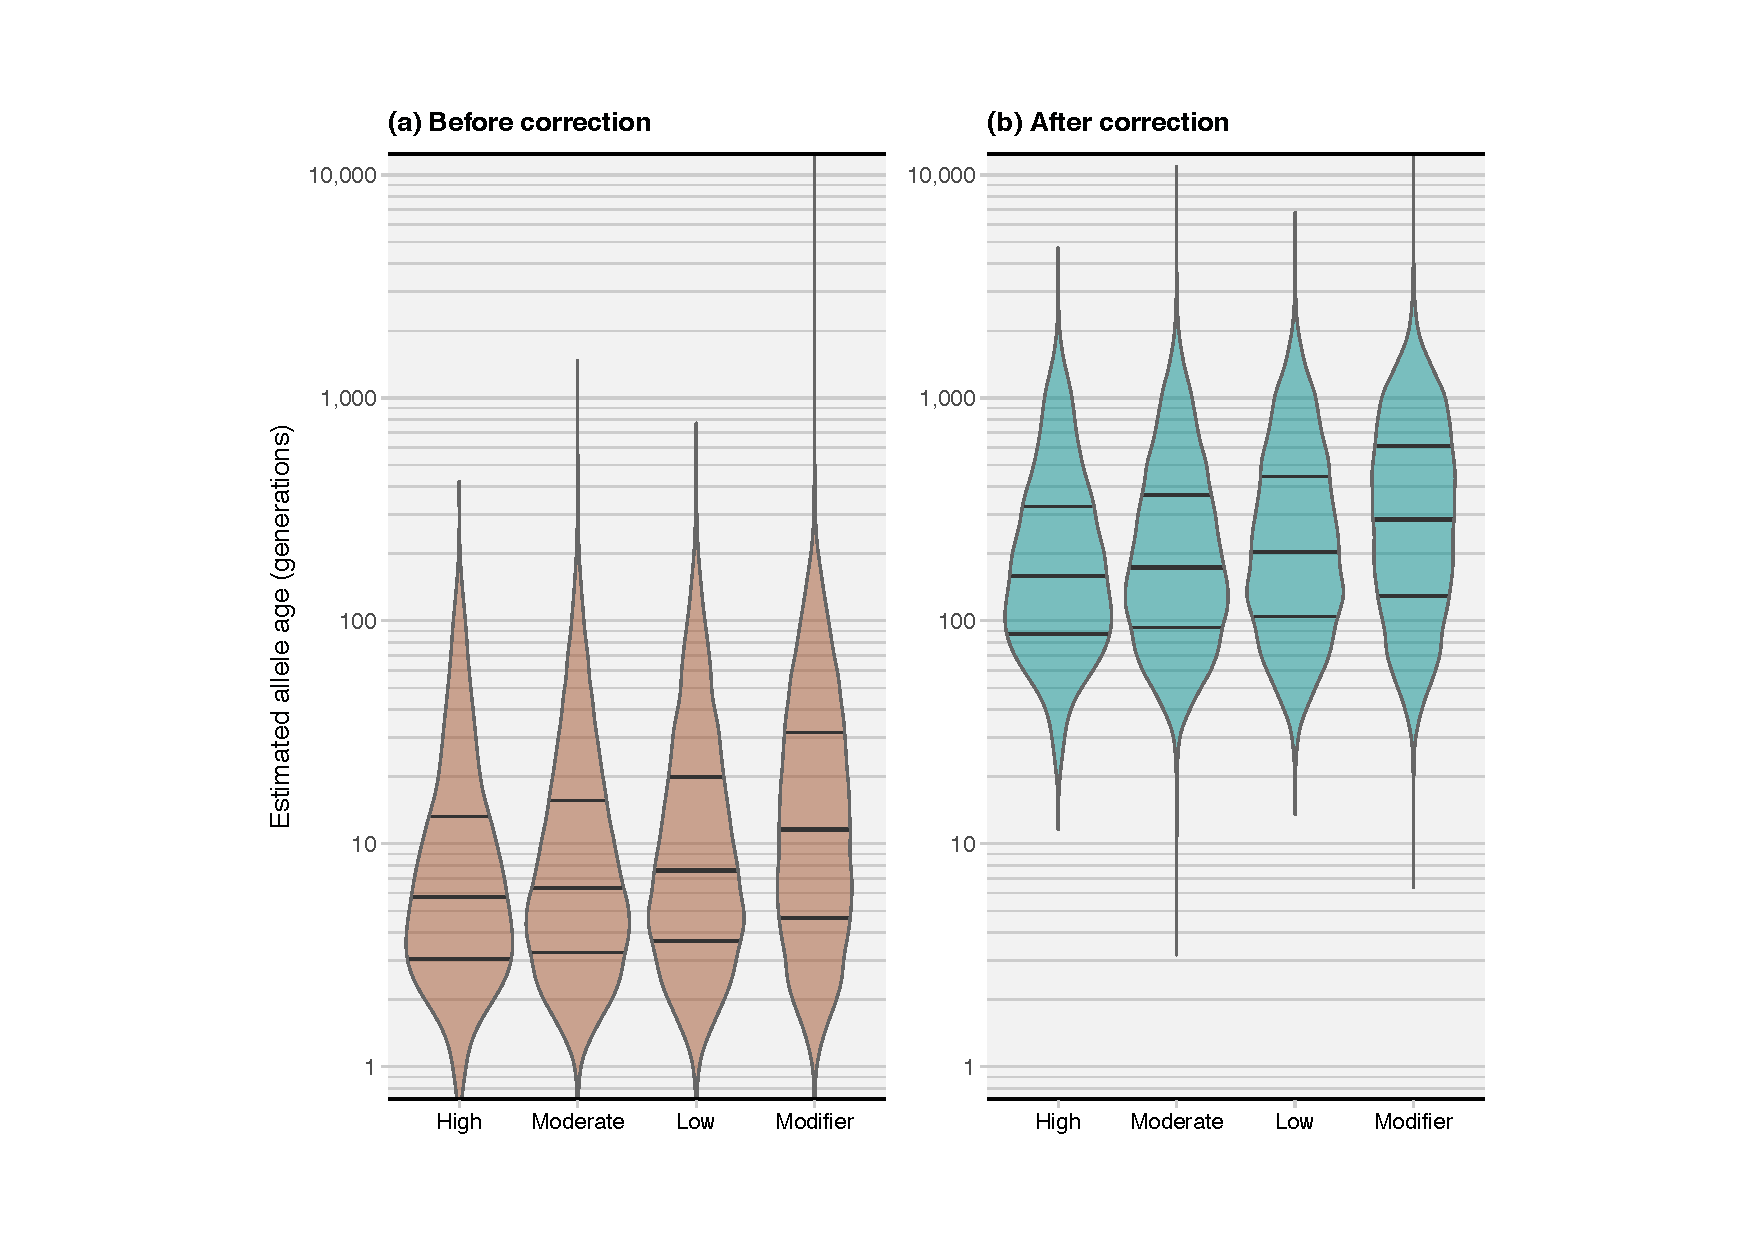
\includegraphics[width=0.75\textwidth]{./img/ch5/1kg_age_impact}
\Caption{Allele age estimated on functionally annotated data in 1000 Genomes}%
{The distribution of inferred allele age is shown in Violin plots by predicted impact category for the whole sample of the \gls{1kg} dataset, before and after correction; \nth{1}, \nth{2}, and \nth{3} quartiles are indicated.}%
{fig:1kg_age_impact}
\end{figure}

%

The number of retained estimates was \n{141069}, which included
\n{1255}~variants of \emph{high} impact (splice acceptor and splice donor variants, and stop gained and stop lost variants),
\n{44131}~variants with \emph{moderate} impact (missense variants only),
\n{9990}~variants with \emph{low} impact (synonymous variants only), and
\n{85694}~\emph{modifier} variants (non-coding variants, \eg intron and intergenic variants, and regulatory region variants).

The distribution of allele age before and after correction is shown in \cpref{fig:1kg_age_impact}.
Before correction, median ages per category were inferred at \numlist{5.6606;6.3292;7.5674;11.8284} generations in \emph{high}, \emph{moderate}, \emph{low}, and \emph{modifier}, respectively, which were corrected to
\numlist{158.1629;174.4351;203.9523;289.5565} generations, respectively.
The correlation between estimated age and allele frequency was measured using $r_S$, which was \numlist{0.829272;0.834355;0.850943;0.867078} in \emph{high}, \emph{moderate}, \emph{low}, and \emph{modifier}, respectively.
Although differences were small, this suggested that the estimated allele age was less correlated with allele frequency if the severity of the presumed consequences was high.

%
%!TEX root = ../../main.tex


\begin{figure}[p]
{\footnotesize\texthv{\textbf{(a) All alleles analysed}}} \\
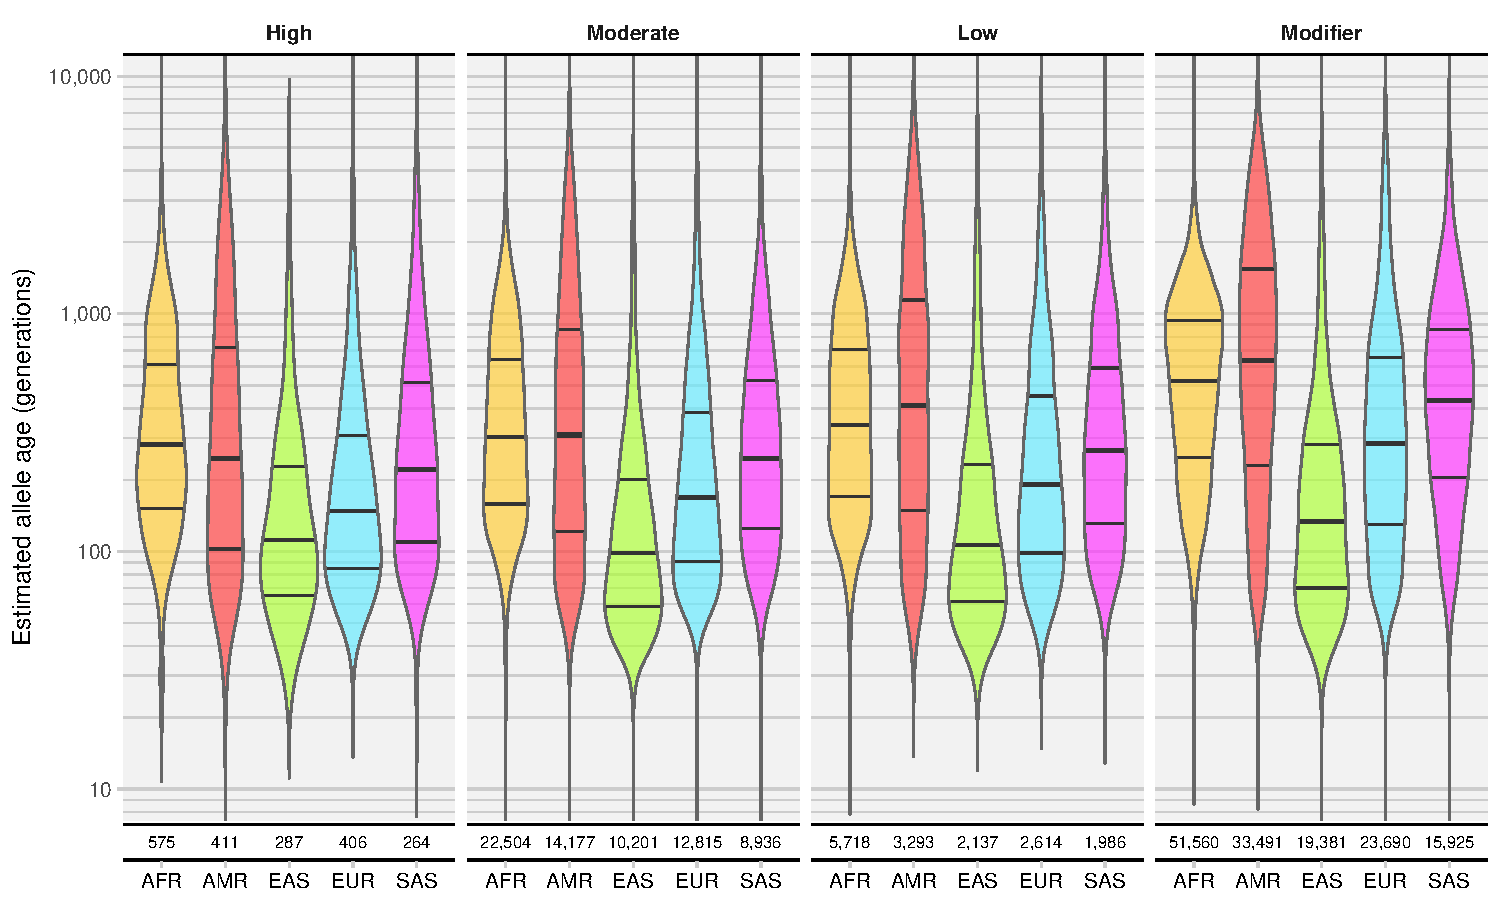
\includegraphics[width=\textwidth]{./img/ch5/1kg_pop_impact_a}
{\footnotesize\texthv{\textbf{(b) Population-specific alleles}}} \\
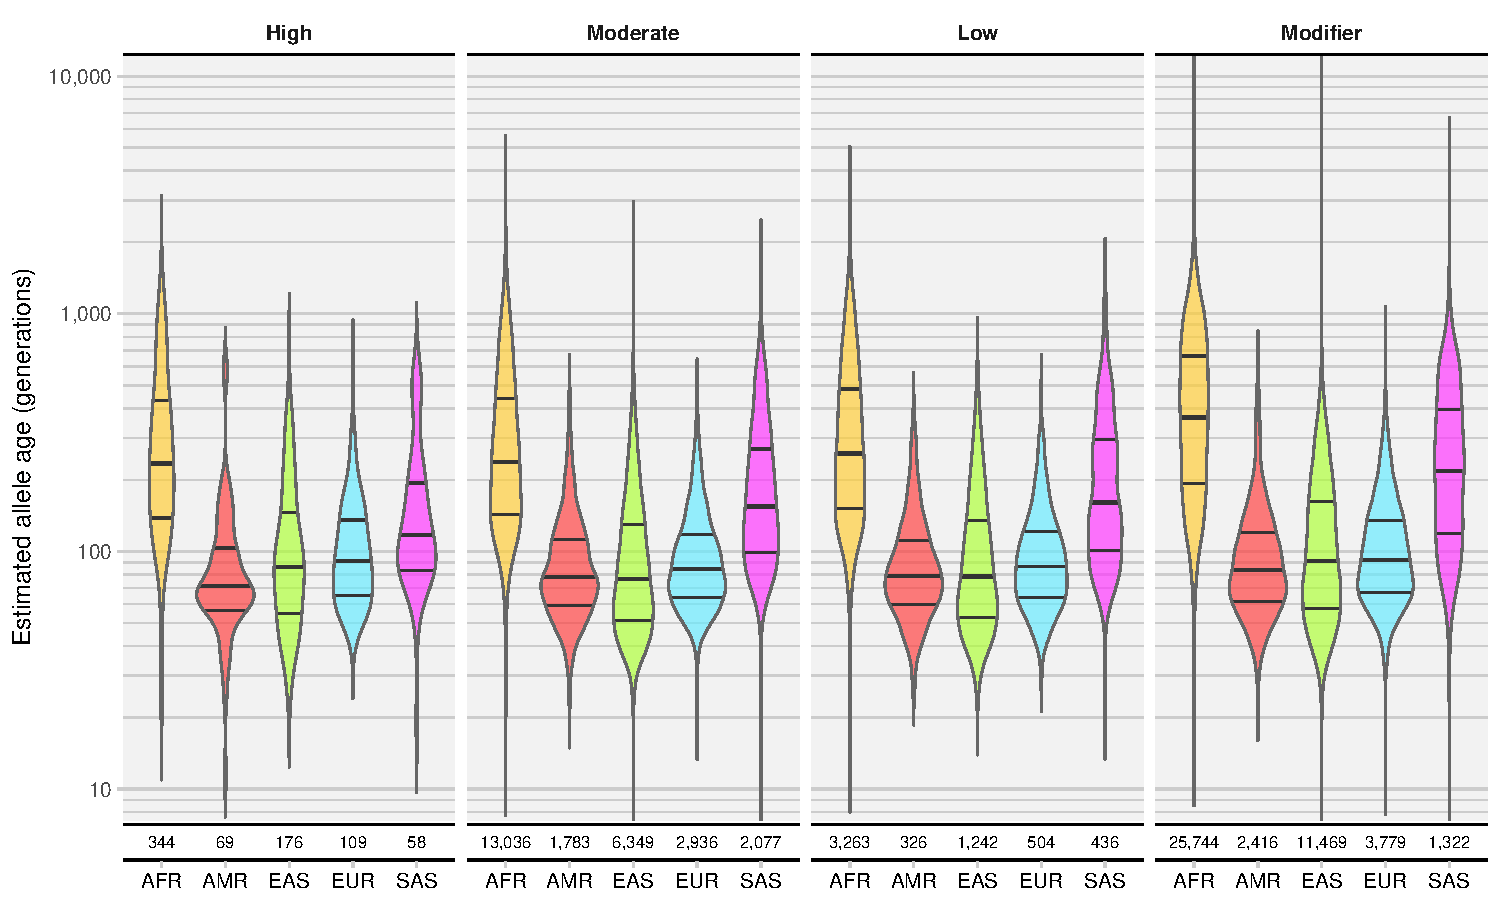
\includegraphics[width=\textwidth]{./img/ch5/1kg_pop_impact_b}
\Caption{Allele age after correction on population-specific frequency in 1000 Genomes}%
{The distribution of inferred allele age is shown in Violin plots by predicted impact category for each population in the \gls{1kg} dataset; \nth{1}, \nth{2}, and \nth{3} quartiles are indicated.
In Panel~\textbf{(a)}, all variants retained after quality control were included in the comparison, which included ${n = \num{141069}}$ target sites.
Note that this also included alleles shared among populations.
In Panel~\textbf{(b)}, only the subset of population-specific variants was included (${n = \num{77438}}$).
The number of alleles retained in each impact category and population are shown below each graph.
The colours used follow the \gls{1kg} colour-scheme.}%
{fig:1kg_pop_impact}
\end{figure}

%

The \gls{1kg} dataset is composed of several continental population samples (or \emph{super-populations}) in which allele frequencies may differ.
I applied the correction as per frequency observed in each population; variants were excluded if monomorphic per population.
Although target sites were selected at ${\leq 1\%}$ allele frequency in the whole sample, some alleles were found at relatively high frequencies in certain populations, but which did not exceed ${5\%}$ allele frequency.
The distribution of allele age per population is shown in \cref{fig:1kg_pop_impact}{a}.
Variants of \emph{high} impact were overall estimated to be younger, \eg median age was \dec{276.7156} generations in AFR and \dec{113.8948} generations in EAS.
Non-coding variants, \emph{modifiers}, were older throughout, \eg \dec{528.8116} generations in AFR, but were not notably older in EAS, where median age was \dec{135.3479} generations.
Alleles in the AMR sample were overall more widely distributed and indicated an older median age per impact category.
Rank correlation with allele frequency, $r_S$, was high in AFR (\dec{0.73132}), but not substantial in EAS (\dec{0.43870}), EUR (\dec{0.40936}), and SAS (\dec{0.34668}).
In AMR, age and frequency appeared to be weakly related (\dec{0.09236}), which may be the result of population admixture, which characterises this population sample.

%
% !TEX root = ../../main.tex


\begin{table}[!htb]
\Caption{Allele age per population in the 1000 Genomes sample}
{Inferred allele age was corrected in reference to population allele frequencies in the \n{5} population groups in \gls{1kg} data, shown per \gls{vep} impact category.
In total, \n{141070} variants were analysed \textbf{(a)}, of which \n{77439} were population-specific \textbf{(b)}.}
{tab:stats_1kg_impact}
\centering
\begin{tabular}{l*5{S[round-precision=1,table-format=3.1]}*5{S[table-format=1.3]}}
	\toprule
	 Impact & \multicolumn{5}{c}{Median estimated age (generations)} & \multicolumn{5}{c}{Correlation with frequency ($r_S$)} \\
	\cmidrule(lr){2-6}
	\cmidrule(lr){7-11}
	 & {AFR} & {AMR} & {EAS} & {EUR} & {SAS} & {AFR} & {AMR} & {EAS} & {EUR} & {SAS} \\
	\otoprule
	\multicolumn{11}{@{\,}l}{(a) All alleles analysed} \\
	\midrule
	\textit{High    } &  276.7156 & 238.2880 & 113.8948 & 145.7969 & 219.0302  &  0.697134 & 0.164036 & 0.444797 & 0.581463 & 0.441301 \\
	\textit{Moderate} &  305.1702 & 311.4755 &  99.0084 & 169.0662 & 247.7381  &  0.707347 & 0.143252 & 0.432302 & 0.469482 & 0.385978 \\
	\textit{Low     } &  341.4061 & 413.9554 & 105.0124 & 191.9495 & 266.3468  &  0.737771 & 0.116200 & 0.388013 & 0.445391 & 0.410477 \\
	\textit{Modifier} &  528.8116 & 645.6322 & 135.3479 & 287.2691 & 435.3400  &  0.728619 & 0.058309 & 0.435299 & 0.349477 & 0.339951 \\
	\otoprule
	\multicolumn{11}{@{\,}l}{(b) Population-specific alleles} \\
	\midrule
	\textit{High    } &  227.2396 & 67.6673 & 86.8637 & 87.8490 & 116.6994  &  0.885856 & 0.672827 & 0.860747 & 0.738088 & 0.864570 \\
	\textit{Moderate} &  239.8254 & 77.3700 & 76.8140 & 84.6032 & 154.8731  &  0.891540 & 0.647132 & 0.877686 & 0.745509 & 0.906612 \\
	\textit{Low     } &  256.4403 & 78.0054 & 77.9945 & 87.1812 & 154.9337  &  0.904668 & 0.616386 & 0.880905 & 0.751465 & 0.907093 \\
	\textit{Modifier} &  369.7328 & 82.7324 & 91.8433 & 91.8594 & 221.5612  &  0.919745 & 0.706728 & 0.896563 & 0.807821 & 0.934936 \\
	\bottomrule
\end{tabular}
\end{table}

%

Variants that appeared in more than \n{1} population were removed to focus on population-specific, presumably more recent alleles; see \cref{fig:1kg_pop_impact}{b}.
This reduced the number of alleles to \n{77438}.
Notably, alleles retained in AMR were youngest in all impact categories, whereas the alleles specific to the AFR sample were seen to be the oldest; \eg median age was \dec{227.2396} generations in \emph{high} and \dec{369.7328} generations in the \emph{modifier} category.
Rank correlation between between allele frequency and inferred age showed a more consistent relationship in each population;
AFR (\dec{0.91654}), EAS (\dec{0.89046}), EUR (\dec{0.77979}), SAS (\dec{0.92096}).
Notably, the variants specific to AMR now showed a moderately high correlation between age and frequency (\dec{0.67690}).
These results are summariesed in \cpref{tab:stats_1kg_impact}.




%
\section{Discussion}
%


% method to narrow down discordant pairs by finding nearest neighbours in outgroup

% outlier identification; inferred IBD lengths that appear to deviate markedly from lengths detected for other pairs that share the same focal allele; separately for concordant and discordant pairs

I demonstrated the validity of the age estimation framework using simulated data where I showed that age can be estimated with very high accuracy.
However, certain problems may arise when working with real data.
The impact of phasing error is small in comparison to genotypic (or allelic) misclassification, which is likely to bias the estimation process.

Generally, imperfect data may affect the estimation of allele age in \n{2} ways.
First, the method was shown to be highly susceptible to inaccurate IBD inference, where each clock model behaves differently to the over or underestimation of IBD length.
In this regard, the \gls{hmm}-based approach for IBD inference was shown to maintain consistency even if genotype error is present.
However, second, even if IBD is detected with high accuracy, the alleles observed at a focal variant in the sample may wrongly identify haplotype sharing by descent.
To account for the possibility that some concordant pairs may actually be discordant pairs, for example, a separate filtering method would be needed to exclude pairs before or after the computation of the \gls{ccf}, to reduce the chance that the calculation of the composite likelihood is biased.
However, because such a method would effectively predict missed alleles in the data, a solution to this problem may not be straightforward.
Yet it would be possible, for example, to exclude pairs on basis of patterns of allele sharing or consistency of the inferred IBD structure.
Alternatively, instead of excluding pairs, the target site itself would need to be excluded from the analysis if bias is likely.
A simple solution was presented in the previous section, where sites are excluded if the lower and upper bounds indicate a reverse order, but further evaluation is required to determine the effectiveness of this filtering criterion.

Lastly, note that both the \gls{dgt} and the \gls{hmm}-based approach operate on genotype data to detect IBD, but because the mutation clock model, \ClockM, requires haplotypes, it would be desirable to estimate pairwise differences, $S$, in genotype data, so as to make these methods fully compatible with \ClockM and \ClockC.
A possible solution is presented in Chapter~3, where haplotype phase was determined from genotype pairs in detected IBD segments, based on the genealogical constrains that arise under haplotype sharing by descent.
Yet, further work is needed to determine the feasibility of such an approach.




% First, correct age estimation may be affected due to its reliance on correct IBD inference, where inaccurate detection of IBD segments was shown to affect the estimation differently under each of the \n{3} clock models.
% Second, even if IBD is detected with high accuracy, the alleles observed at a focal variant in the sample may wrongly identify individuals through
% haplotype sharing may not be
% a focal allele may incorrectly identify haplotype sharing in the sample.
% In particular, the \n{2} types of error are \emph{false positives} (Type~1 error), where an allele wrongly identifies haplotype sharing, and \emph{false negatives} (Type~2 error), where an allele was missed.
% Both types affect

% misclassified alleles along the shared sequence may artificially inflate the genetic length number of pairwise differences, $S$, seen between haplotype sequences, which affects both the mutation clock, \ClockM, and the combined clock, \ClockC.
% I showed that the impact of phasing error is small compared to genotype error, which is relevant when the \gls{fgt} is used for IBD detection.
% When the \gls{dgt} or the \gls{hmm}-based approach is used, the misclassification of genotypes is the main source of error.
% Third, the analysis is likely to be biased if the alleles observed at a target site incorrectly identify haplotype sharing in the sample.



% \begin{description}
% 	\item[\textbf{Type \rom{1}}] errors or \emph{false positives}
% 	\item[\textbf{Type \rom{2}}] errors or \emph{false negatives}
% \end{description}
